\documentclass[11pt]{article}

% Preamble for writeup_v3.
% Shared packages, fonts, hyperref config, and notation shortcuts.

\usepackage{amsmath, amssymb}
\usepackage{geometry}
\usepackage{graphicx}
% Figures live at chain-model/figures/ and chain-model/figures/panels/;
% this file is at chain-model/writing/writeup_v3/, so paths are two levels up.
\graphicspath{{../../figures/}{../../figures/panels/}}
\usepackage{hyperref}
\usepackage{xcolor}
\usepackage{booktabs}
\usepackage{enumitem}

\geometry{margin=1.2in}

\hypersetup{
    colorlinks=true,
    linkcolor=blue!60!black,
    citecolor=blue!60!black,
    urlcolor=blue!60!black
}

% Match the figure typography: Computer Modern Sans Serif throughout.
\renewcommand{\familydefault}{\sfdefault}
\usepackage[T1]{fontenc}

% Notation shortcuts.
\newcommand{\Nzero}{N_0}
\newcommand{\bEdge}{b_e}
\newcommand{\dEdge}{d_e}
\newcommand{\bCore}{b_c}
\newcommand{\dCore}{d_c}
\newcommand{\bR}{b_R}
\newcommand{\dR}{d_R}
\newcommand{\sR}{s_R}
\newcommand{\sE}{s_e}

% Inline TODO marker for stub sections.
\newcommand{\TODO}[1]{\textcolor{red}{\textbf{[TODO: }#1\textbf{]}}}


\title{Spatial rescue in biofilms:\\
a double-edged sword}
\author{}
\date{\today}

\begin{document}
\maketitle

\begin{abstract}
\noindent A biofilm under antibiotic treatment has a clear spatial
asymmetry: cells on the surface are exposed to the drug, while cells
in the deeper interior are shielded from it. We ask whether that
shielded interior makes the population more likely to evolve drug
resistance and survive, a process known as evolutionary rescue.
Comparing a spatially structured biofilm model against a well-mixed
population of the same initial size, and sweeping the antibiotic dose
along with the metabolic activity of the interior, we find that the
biofilm is a double-edged sword; it rescues less often than
the well-mixed reference at low dose, but more often at high dose,
and only when the interior is metabolically active. We explain this pattern as a consequence of two opposing effects of the spatial structure: a supply mechanism that generates resistant mutants in the interior yet is subject to drift since it is not exposed to the drug, and a delivery mechanism that transports those mutants to the surface where they can grow and establish but is tied to antibiotic dose via the velocity at which the biofilm deteriorates. Our results suggest that the spatial structure of biofilms can both hinder and facilitate evolutionary rescue, and that the balance between these effects depends on the antibiotic dose and the metabolic activity of the interior.

\end{abstract}

\section{Introduction}
\label{sec:intro}

Antibiotic resistance is an escalating clinical problem, and biofilms (dense, surface-attached bacterial communities) carry a disproportionate share of it. Biofilms are responsible for a large fraction of chronic infections and are notoriously hard to clear with antibiotics; standard regimens that work in well-mixed culture often fail when the target population is organized as a biofilm. This has driven interest in behavior-modifying interventions, in particular compounds that induce bacterial dispersal away from biofilms toward a planktonic, or more well-mixed state. Such interventions do not kill cells; they simply change how cells are arranged in space. The hope is that disrupting biofilm spatial structure reduces the population's capacity to evolve resistance under antibiotic pressure, essentially disarming the bacteria such that they will be more easily cleared by traditional antibiotic treatments and the host immune system. Knowing whether that hope is justified requires understanding what the spatial structure of a biofilm actually does to a population's evolutionary dynamics in the first place. Does biofilm formation help the population evolve resistance, hurt it, or some combination of both?

Biofilms have a clear spatial asymmetry: cells on the outer surface are exposed to the drug, while cells in the deeper interior are shielded from it. The shielded interior is a spatial refuge, a region of the population where the antibiotic selection pressure does not reach. We ask whether that refuge makes the population more likely to undergo \emph{evolutionary rescue}, the outcome in which a declining population avoids extinction because a resistant mutant arises and takes over in time. Concretely: does a biofilm with a shielded interior rescue more often than a well-mixed population of the same initial size?

The naive prediction is that the refuge provided by biofilm structures should help facilitate evolutionary rescue. The biofilm creates a gradient of antibiotic concentration, with the shielded interior experiencing lower levels of the drug. This shielded interior lets the population persist for longer under treatment, and a longer overall population-level lifespan means more cell divisions, which means more opportunities for a resistant mutation to arise. More mutations should mean more rescue. But this prediction has at least two distinct ways it could be wrong. First, a mutation that arises in the shielded interior does nothing on its own: there is no selection pressure inside the refuge to make a resistant cell take over, so a core mutation matters only if it eventually reaches the drug-exposed surface in time to grow under selection. The refuge might generate mutations the population can never actually use. Second, the very mechanism that maintains the refuge, namely the replacement of dying surface cells by cells flowing outward from the interior, could act against a new resistant cell trying to establish on the surface by ensuring it is surrounded by a continuously refreshed wild-type majority. The same spatial structure that buys extra time may also make each individual mutation that arises less useful. Whether the biofilm is a net help or a net hindrance therefore depends on how these effects balance.

We measure that balance directly by simulating a minimum-viable biofilm (a one-dimensional chain of cells with a drug-exposed edge and a shielded core) under antibiotic pressure, and compare its rescue probability against an otherwise identical well-mixed population. By varying the antibiotic dose and the metabolic activity of the interior independently, we ask whether the biofilm's spatial structure is uniformly helpful, uniformly harmful, or, as the results below will show, contingent on both the selection pressure and on what is happening inside the refuge.

\section{The model}
\label{sec:model}

We model the biofilm as a one-dimensional chain of cells. Real biofilms are three-dimensional, but the central asymmetry we are after (drug-exposed surface versus shielded interior) does not need three dimensions to capture. One dimension keeps the dynamics tractable while preserving the feature that matters: cells at different positions face different antibiotic concentrations.

\subsection{The chain and rates}
\label{ssec:chain}

The state of the population at any time $t$ is an ordered list of cells indexed $0, 1, \ldots, N(t) - 1$. Index $0$ is the deep interior; index $N(t) - 1$ is the outer surface. Each cell has a genotype, either wild-type (WT) or resistant (R), and a position determined by its index. As per convention with evolutionary rescue, the population starts at $t = 0$ with $N(0) = \Nzero$ WT cells and no resistant cells. The population then evolves under antibiotic pressure, which begins at time $t = 0$, with births and deaths changing the chain's length and composition over time. 

Antibiotic exposure is a step function in position. At any given population size $N(t)$, the rightmost $l$ cells of the chain form the edge, the region where antibiotic concentration is lethal to WT. In this model, we assume $l$ to be a fixed integer parameter describing the width of the edge, or the thickness of the drug-exposed layer. All cells with index $< N(t) - l$ form the core, the shielded interior. The boundary between edge and core sits at position
\begin{equation}
b(t) \;=\; \max\bigl(0,\, N(t) - l\bigr),
\label{eq:boundary}
\end{equation}
so as the population shrinks, the boundary retreats from the surface toward the interior. When $N(t) \le l$ the boundary collapses to $b = 0$, and the entire population is edge; no core remains. Additionally, the well-mixed equivalent of this model is the special case where $l \ge \Nzero$, so the edge is as wide as the entire population and there is no core at all. The boundary is always at $b = 0$ in that case, and every cell is drug-exposed from the start. The flat step-function profile is a stylization of the real, smooth antibiotic gradient through a biofilm. Treating the boundary as sharp is the minimum-viable abstraction that captures the asymmetry; so it is reasonable to assume that a smooth gradient would change quantitative numbers but not the qualitative dynamics we are after.

Each cell has a birth rate and a death rate determined by its compartment and its genotype, summarized in Table~\ref{tab:rates}.

\begin{table}[htbp]
\centering
\small
\begin{tabular}{lcccc}
\toprule
                & \multicolumn{2}{c}{Core ($i < b$)} & \multicolumn{2}{c}{Edge ($i \ge b$)} \\
\cmidrule(lr){2-3} \cmidrule(lr){4-5}
                & birth        & death        & birth        & death \\
\midrule
Wild-type (WT)  & $\bCore$     & $\dCore$     & $\bEdge$     & $\dEdge$ \\
Resistant (R)   & $\bCore$     & $\dCore$     & $\bR$        & $\dR$ \\
\bottomrule
\end{tabular}
\caption{Per-cell birth and death rates by compartment and genotype, where $i$ is the cell index in the chain, and $b(t)$ is the boundary position between core and edge. The eight compartment-genotype-event combinations that drive the Gillespie dynamics are described in \S\ref{ssec:dynamics}.}
\label{tab:rates}
\end{table}

The edge WT birth rate $\bEdge = 1$ sets the time unit, where time is tracked in generations as the inverse of the birth rate $\frac{1}{\bEdge} = 1$. The edge WT death rate $\dEdge$ is the antibiotic dose, swept over values $\dEdge > \bEdge$ so WT cells in the edge are always net-dying under treatment. Resistant cells in the edge have $\bR = 1$ and $\dR = 0.6$, giving them a positive net growth rate $\sR = \bR - \dR = 0.4$ once they reach the drug-exposed surface; an R lineage that establishes in the edge grows deterministically to dominance. Notably, however, there are different classes of antibiotic, and some drugs are bacteriostatic rather than bactericidal. For a bacteriostatic drug, the edge WT death rate would be $\dEdge = \bEdge = 1$, so WT cells in the edge would be net-neutral rather than net-dying. We do not study that case here, but it is straightforward and possibly interesting to implement by setting $\dEdge = 1$. \footnote{We would expect that if WT cells were stalled in growth but not dying, rescue dynamics would be different.} Additionally, the model allows multiple $R$ lineages to arise and compete, but the assumptions are such that rescue is defined whenever there are at least $r_{\mathrm{thr}} = 10$ R cells in the edge, so the first lineage or combination of lineages to reach that threshold is what determines rescue. As such, we do not examine the dynamics of clonal interference among $R$ lineages, which would be an interesting topic for future work but is not the focus here.

Cells in the core, regardless of genotype, have balanced rates $\bCore = \dCore$. The core has no net growth on its own, and WT and R are treated identically there because the shielded interior carries no selection. The default core rate is $\bCore = 0.2$, a slow but nonzero pace; the dormant-core limit is $\bCore = 0$, where the interior produces no births and no deaths at all. Comparing these two limits is one of the central experiments below.\footnote{To prevent unbounded post-rescue growth, R births in both compartments are multiplied by a Wilson-type density factor $\max(0,\, 1 - N/K)$, with $K = \Nzero$ throughout. WT births stay density-independent. The factor is approximately $1$ during the wild-type decline that we study, so it does not affect the dynamics of interest; it matters only once R has taken over.}

\subsection{Dynamics}
\label{ssec:dynamics}

Events fire one at a time, sampled as a continuous-time Markov chain via the Gillespie algorithm. At each step we compute the total event rate $R_{\mathrm{tot}}$ across all eight compartment-genotype-event combinations in Table~\ref{tab:rates}, advance simulated time by an exponential draw with mean $1/R_{\mathrm{tot}}$, and pick which event fires from a categorical distribution with weights proportional to each event's rate.

A birth event picks a parent uniformly at random within its compartment-genotype subgroup. The daughter is inserted adjacent to the parent (at the parent's position or one position to the right, each with probability $1/2$), and the chain grows by one. A death event picks a victim uniformly at random within its subgroup and removes it; the chain contracts by one.

The boundary $b(t)$ is recomputed after every event according to Eq.~\eqref{eq:boundary}. When the population grows by one and the boundary moves outward, the cell that now sits at the new boundary position has crossed from edge into core; it is reclassified as a core cell. When the population shrinks and the boundary moves inward, the cell that now sits one position outside the new boundary has crossed from core into edge; it is reclassified as an edge cell. These reclassifications are not separate dynamical events: they are bookkeeping consequences of recomputing the boundary against a chain that has just changed length by one.

This bookkeeping is the \emph{conveyor belt} mechanism the rest of the writeup will refer to. As long as the core has cells in it, every edge death pulls an interior cell out to the surface, and every edge birth pushes an outer cell back into the interior. The result is that the edge holds exactly $l$ cells while the core has anything left to supply; the population is shrinking, but the surface layer is being continuously replaced from below. Figure~\ref{fig:conveyor}(a, b) illustrates one such reclassification on a small didactic chain: a cell in the same physical position is in the core before an edge death and in the edge after, because the boundary has moved over it.

\begin{figure}[h!]
\centering
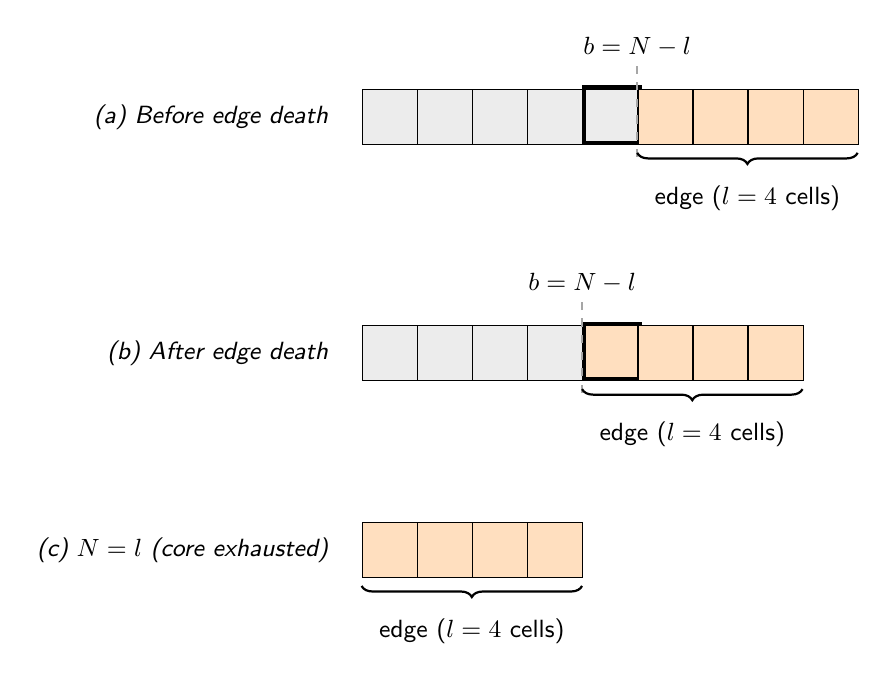
\begin{tikzpicture}[
    every node/.style={font=\small},
    cellbox/.style={draw=black, line width=0.5pt, minimum width=0.7cm, minimum height=0.7cm, anchor=south west},
    corecell/.style={cellbox, fill=gray!15},
    edgecell/.style={cellbox, fill=orange!25},
    tracked/.style={line width=1.6pt},
    bracket/.style={decorate, decoration={brace, amplitude=4pt, mirror}, thick},
    boundary/.style={dashed, gray!70, thick},
    panellabel/.style={anchor=east, font=\small\itshape},
]

% Panel (a). N = 9, l = 4, so b = 5. Tracked cell at position 4 (innermost core).
\node[panellabel] at (-0.3, 3.35) {(a) Before edge death};

\foreach \i in {0,1,2,3} {
  \node[corecell] at (\i*0.7, 3.0) {};
}
\node[corecell, tracked] at (4*0.7, 3.0) {};
\foreach \i in {5,6,7,8} {
  \node[edgecell] at (\i*0.7, 3.0) {};
}

\draw[boundary] (3.5, 2.85) -- (3.5, 4.0);
\node[above, font=\small] at (3.5, 4.0) {$b = N - l$};

\draw[bracket] (3.5, 2.9) -- (6.3, 2.9)
  node[midway, below=8pt, font=\small] {edge ($l=4$ cells)};

% Panel (b). N = 8, l = 4, so b = 4. The tracked cell, same physical
% position, has been reclassified into the edge.
\node[panellabel] at (-0.3, 0.35) {(b) After edge death};

\foreach \i in {0,1,2,3} {
  \node[corecell] at (\i*0.7, 0.0) {};
}
\node[edgecell, tracked] at (4*0.7, 0.0) {};
\foreach \i in {5,6,7} {
  \node[edgecell] at (\i*0.7, 0.0) {};
}

\draw[boundary] (2.8, -0.15) -- (2.8, 1.0);
\node[above, font=\small] at (2.8, 1.0) {$b = N - l$};

\draw[bracket] (2.8, -0.1) -- (5.6, -0.1)
  node[midway, below=8pt, font=\small] {edge ($l=4$ cells)};

% Panel (c). After enough edge deaths, N has fallen to l. The boundary
% collapses to b = 0 and the entire chain is edge.
\node[panellabel] at (-0.3, -2.15) {(c) $N = l$ (core exhausted)};

\foreach \i in {0,1,2,3} {
  \node[edgecell] at (\i*0.7, -2.5) {};
}

\draw[bracket] (0, -2.6) -- (2.8, -2.6)
  node[midway, below=8pt, font=\small] {edge ($l=4$ cells)};

\end{tikzpicture}
\caption{The conveyor belt as a consequence of recomputing the boundary, illustrated on a small didactic chain with $N = 9$ initial cells and $l = 4$. The rightmost $l$ cells (orange) form the edge; the rest (grey) form the core. (a) Before the event, the cell drawn with a heavy outline sits in the core, immediately inside the boundary $b = N - l$. (b) After an outer edge cell has died, $N$ has dropped to $8$ and the recomputed boundary has moved one position inward; the tracked cell, in the same physical position, is now part of the edge. No cell has been shuffled; the bracket has shifted over it. (c) After enough cumulative edge deaths, $N$ reaches $l$: the boundary collapses to $b = 0$, the entire chain is edge, and the dynamics enter Phase 2. An edge birth is the symmetric operation, with the boundary moving outward by one position and the innermost edge cell reclassified as core.}
\label{fig:conveyor}
\end{figure}

The conveyor belt produces two qualitatively different regimes of decline. While the core still has cells in it ($N(t) > l$), each edge death is replaced immediately by a core cell, so the edge stays at exactly $l$ cells. Only the $l$ edge cells contribute to net loss, at rate $\sE \cdot l$ per unit time, and the total population falls linearly, where $\sE = \dEdge - \bEdge$. The duration of this buffered decline is
\begin{equation}
T_1 \;=\; \frac{\Nzero - l}{\sE \cdot l},
\label{eq:T1}
\end{equation}
which is long at low dose (slow edge turnover empties the core gradually) and brief at high dose (fast edge turnover empties the core quickly). Once the core is exhausted ($N(t) \le l$; Figure~\ref{fig:conveyor}(c)), the edge is the entire remaining population, and there is no reservoir to draw on. The remaining $\le l$ cells decay exponentially at rate $\sE$, just as a well-mixed population would. The transition between these two regimes is sharp on the simulation timescale: it happens at the moment the last core cell is converted to edge. After that point, the dynamics on the chain are indistinguishable from those of a one-compartment well-mixed model with $N = l$.

\subsection{Mutations, rescue, and initial condition}
\label{ssec:mutations}

Mutations are replication-linked: at each WT birth event, with probability $\mu$, the daughter is an R cell instead of WT; otherwise the daughter inherits the parent's genotype. Mutations are irreversible (no back-mutation from R to WT), so once a lineage is R, all of its descendants are R. Because mutations ride on births, they appear at specific spatial positions on the chain (the position of the dividing parent); a mutation born deep in the core enters the world at the core's spatial location and must be physically transported to the edge to come under selection.

Every R lineage that ever appears is tagged with a unique identifier when its founder is born, and that identifier propagates to all descendants. This lets us follow each mutation individually: where it was born (core or edge), when it appeared, how its descendant population grew, whether it ever reached the edge, and whether it contributed to rescue. The per-lineage records produced by this tracking are the basis for most of the analyses in later sections.

A run is declared $\mathrm{rescued}$ when the edge contains at least $r_{\mathrm{thr}} = 10$ resistant cells simultaneously. The choice of $r_{\mathrm{thr}} = 10$ is high enough to be well past the establishment bottleneck (the regime where a small R lineage might still go extinct by chance) but small enough that rescue is declared promptly after takeover begins. Once an R lineage is past establishment in the edge, where $\sR > 0$, it grows deterministically to dominance. Every simulation terminates naturally on one of two events: rescue ($\ge r_{\mathrm{thr}}$ R cells in the edge) or extinction ($N = 0$). There are no artificial time or generation caps. Both endpoints are guaranteed by the dynamics: either a successful resistant lineage establishes in time, or the wild-type population is driven to zero. The model cannot stall in between.

Every simulation starts at $t = 0$ with $N = \Nzero$ wild-type cells and no resistant cells. Before $t = 0$ the population is at quasi-steady state, with balanced birth and death rates in both compartments ($\bEdge = \dEdge = 1$ pre-treatment in the edge, $\bCore = \dCore$ in the core), so the biofilm neither grows nor shrinks. At $t = 0$ the antibiotic switches on: the edge WT death rate jumps from $\bEdge = 1$ to its treatment value $\dEdge > 1$, and the population begins to decline. What we simulate is therefore the response of an already-mature biofilm to a step-function antibiotic challenge. Real treatments are gradual; this abstraction strips out the loading dynamics so that the rescue dynamics, the only thing we are studying, are not entangled with growth-phase or pharmacokinetic transients.

\subsection{The well-mixed reference}
\label{ssec:wm}

To say whether the biofilm helps or hurts, we need a baseline. Our baseline is a well-mixed population of the same initial size $\Nzero$, governed by the edge birth and death rates alone: every cell is drug-exposed, none are shielded. This is the standard setting for evolutionary rescue (Wilson et al., 2017), and it is the natural null model, the same biofilm with all spatial structure removed. We simulate this fully well-mixed model (essentially a one-compartment model and faithful recreation of Wilson's evolutionary rescue model). Operationally, however, the true well-mixed reference to our biofilm model is the chain model with $l \ge \Nzero$: when the edge is as wide as the entire population, no cell is ever in the core, the conveyor belt never engages, and the dynamics reduce to a one-compartment birth-death process on scalar counts. We also maintain an independent scalar-count implementation as a cross-check; the two well-mixed models agree statistically within sampling error, which serves as an internal consistency test on the chain model.


\subsection{Parameters and simulation details}
\label{ssec:params}
Unless stated otherwise, all simulations use the parameters in Table~\ref{tab:params}. Time is measured in edge generations ($\bEdge = 1$). The dose sweep covers $\dEdge \in \{1.05,\,1.1,\,1.2,\,1.4,\,1.6,\,1.9,\,2.3,\,2.8\}$. The core-activity sweep covers $\bCore \in \{0,\,0.05,\,0.1,\,0.2,\,0.4,\,0.8\}$. The edge-width sweep covers $l \in \{25,\,50,\,100,\,200,\,400\}$. Every parameter combination is run with $5{,}000$ independent seeds; the well-mixed reference is run at the same dose points with the same seed count.

\begin{table}[h!]
\centering
\small
\begin{tabular}{lll}
\toprule
Parameter & Value & Meaning \\
\midrule
$\Nzero$           & $1000$        & Initial population size \\
$l$                & $100$ (swept) & Fixed value for edge width (\# cells exposed to drug) \\
$\bEdge$           & $1.0$         & WT birth rate in edge (sets time unit) \\
$\dEdge$           & dose (swept)  & WT death rate in edge; super-MIC is $\dEdge > 1$ \\
$\bR$              & $1.0$         & R birth rate in edge \\
$\dR$              & $0.6$         & R death rate in edge ($\sR = 0.4$) \\
$\bCore = \dCore$  & $0.2$ (swept) & Core birth \& death rate ($0$ = dormant) \\
$\mu$              & $10^{-4}$     & Mutation probability per birth \\
$r_{\mathrm{thr}}$ & $10$          & Resistant edge cells required to declare rescue \\
$K$                & $\Nzero$      & Density cap for R births (see footnote, \S\ref{ssec:chain}) \\
\bottomrule
\end{tabular}
\caption{Default model parameters. The swept variables are dose ($\dEdge$), core activity ($\bCore$), and edge width ($l$).}
\label{tab:params}
\end{table}

\section{The double-edged sword}
\label{sec:doubleedge}

Section~\ref{sec:intro} closed with a prediction (the refuge should help) and two distinct ways the prediction could be wrong. The refuge could be useless on its own, with the extra lifetime never translating into extra rescue. Or the refuge could be helpful only under specific conditions, say only when the antibiotic dose is high or only when the interior is metabolically active, so that the average effect across regimes hides a sharp contingency. These are different failure modes, and they imply different things about what spatial structure does for a population trying to evolve resistance. We want to distinguish them in a single experiment.

The cleanest way to do that is to vary two knobs independently. The first knob is the antibiotic dose, which we sweep between a value just above the minimum inhibitory concentration ($\dEdge = 1.05$) and a value well above it ($\dEdge = 2.8$). The second is the metabolic activity of the interior, which we set to two values: $\bCore = 0$ (dormant; the interior is a passive refuge with no births and no deaths) and $\bCore = 0.8$ (active; the interior is dividing at a substantial fraction of the edge rate). At each of the four combinations we run $5{,}000$ independent simulations of the biofilm and $5{,}000$ of the well-mixed reference, and compute the fraction that rescue.

Each of the two knobs isolates a different question. The dormant-core column ($\bCore = 0$) asks whether the geometric refuge by itself matters: with no births in the interior, the only thing the biofilm gains over the well-mixed reference is extra lifetime; does that alone help? The active-core column ($\bCore = 0.8$) asks whether what happens inside the refuge matters: with the interior dividing, the biofilm has extra cell divisions on top of the lifetime extension; do those help? And running both at low and high dose asks whether the answers depend on the selection pressure that is forcing rescue in the first place. Four cells of a $2 \times 2$ design, three live hypotheses tested at once.

\begin{figure}[htbp]
\centering
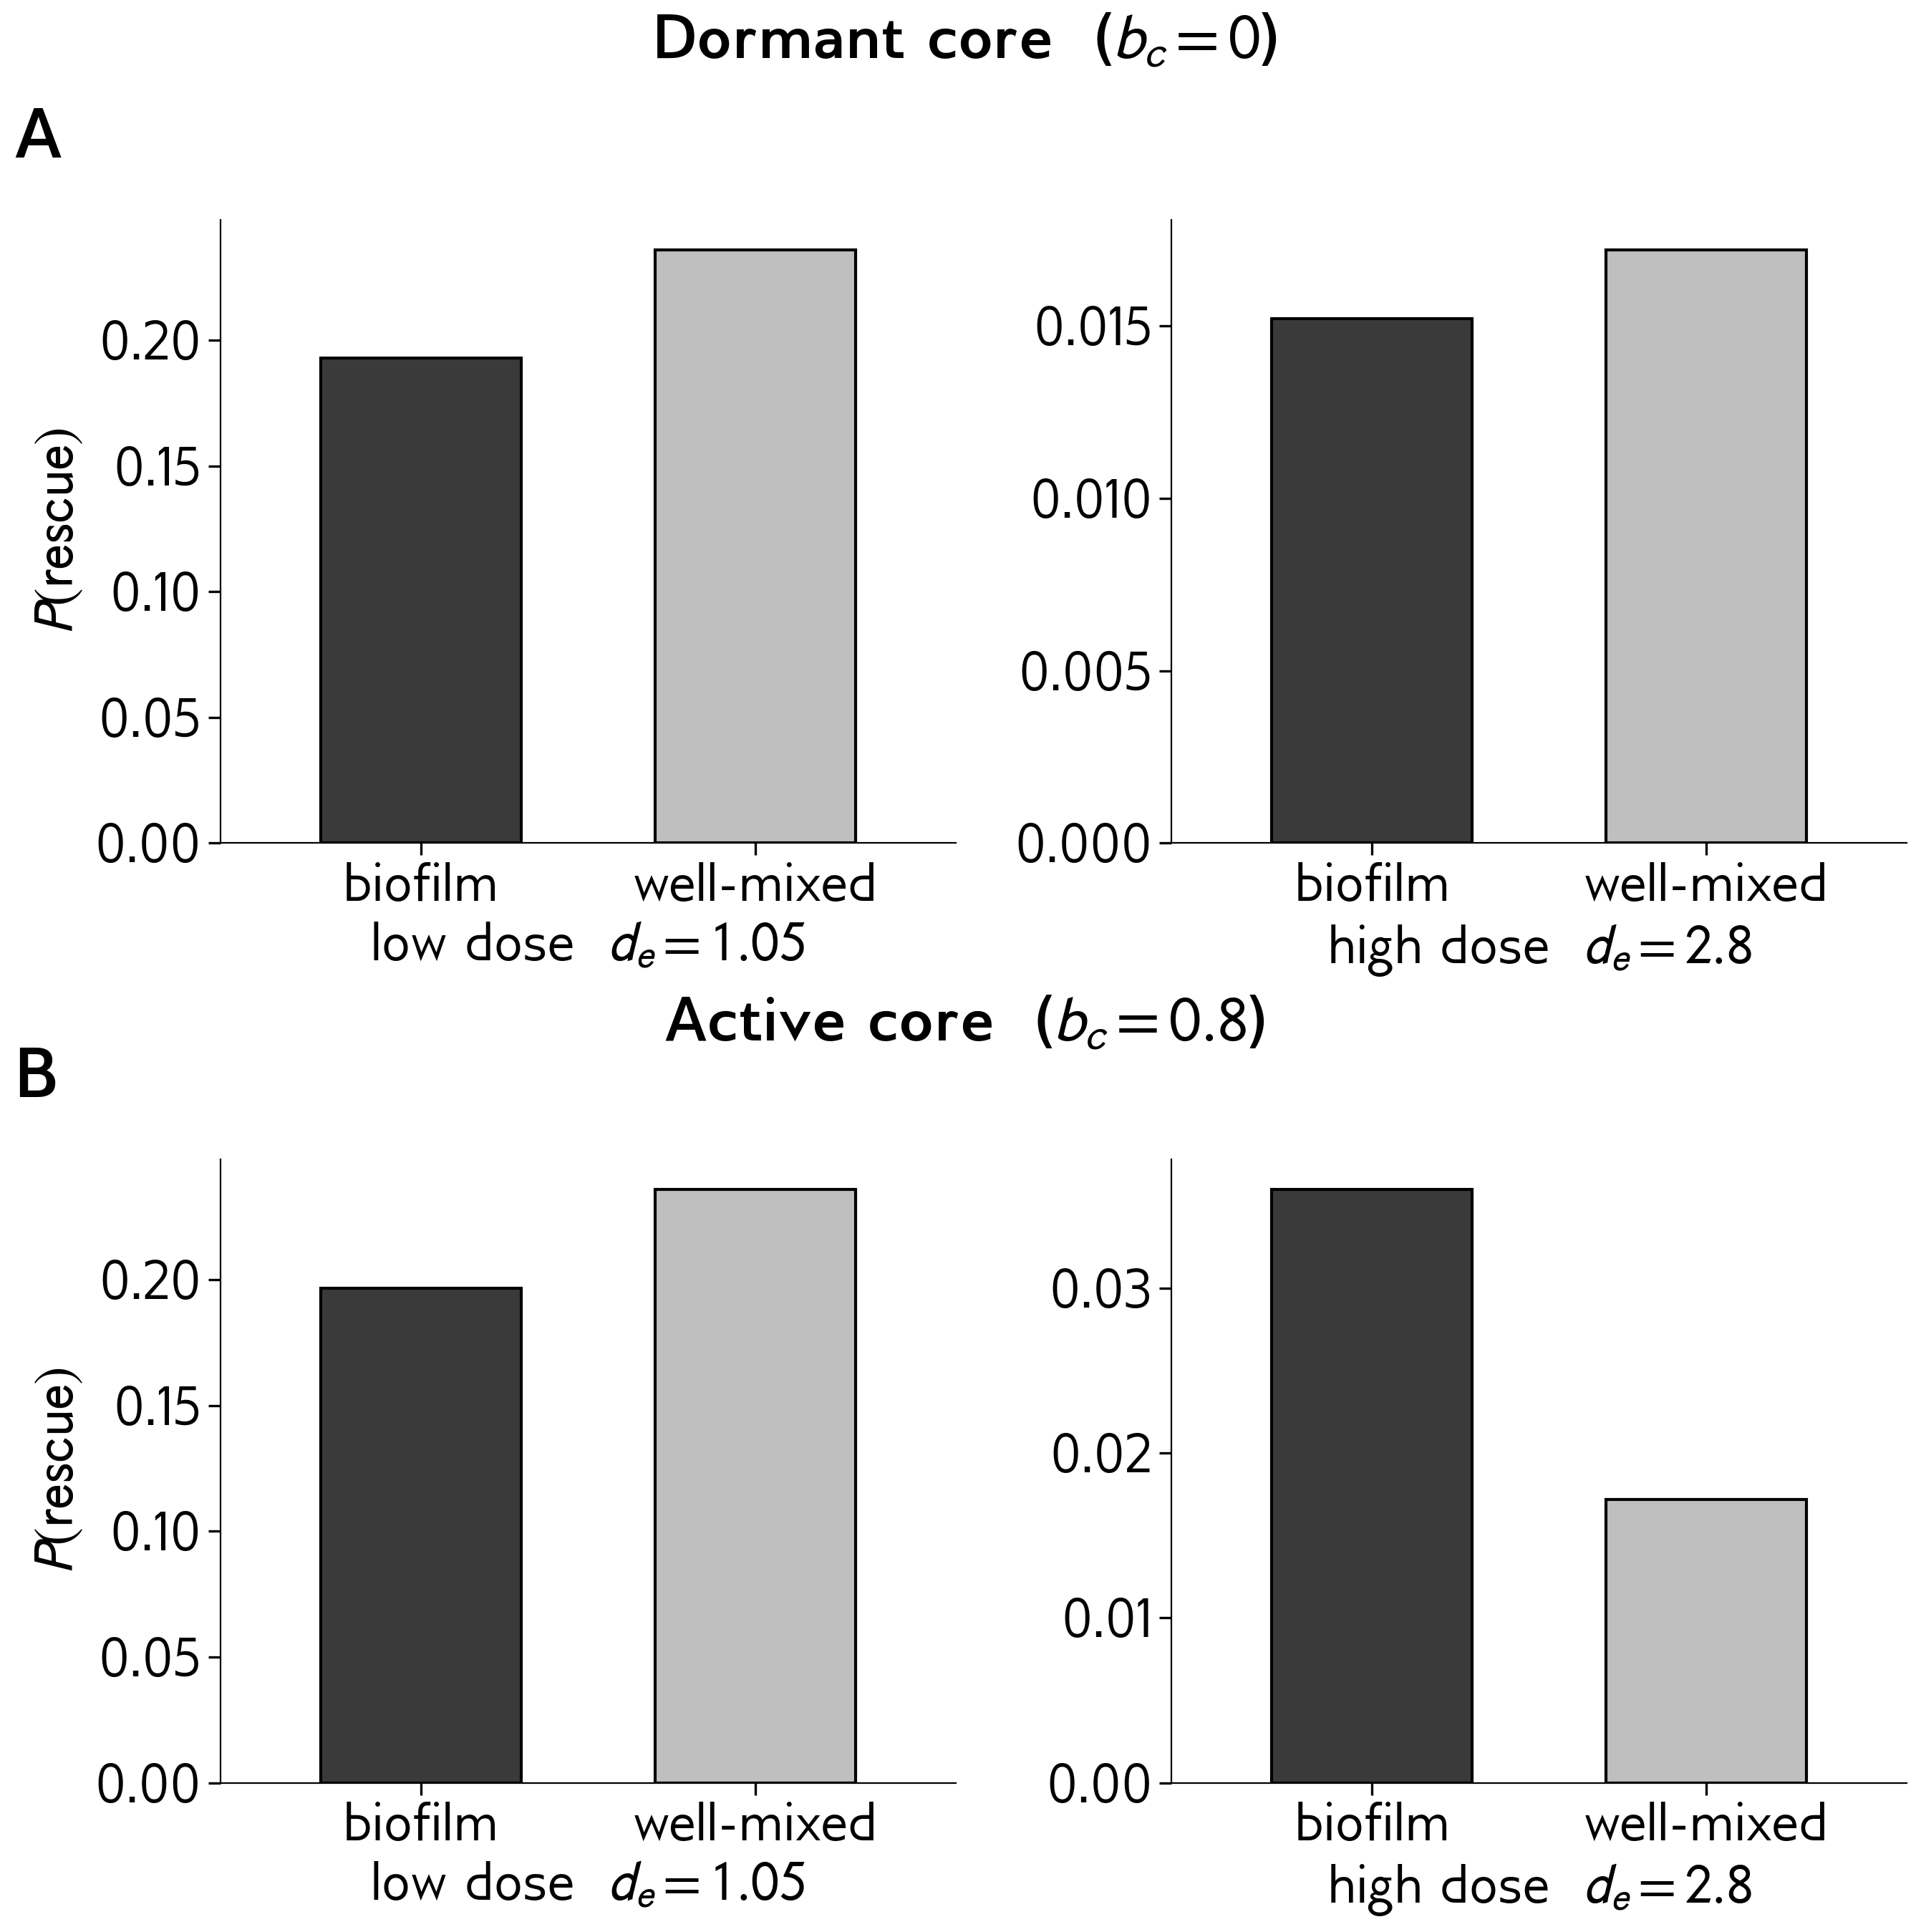
\includegraphics[width=0.75\textwidth]{double_edge_rescue.png}
\caption{Rescue probability for the biofilm (dark) versus the well-mixed reference (light), at low dose ($\dEdge = 1.05$, left columns) and high dose ($\dEdge = 2.8$, right columns). Panel A: dormant core ($\bCore = 0$). Panel B: active core ($\bCore = 0.8$). Each subplot uses its own y-axis scale. \emph{Parameters}: $\Nzero = 1000$, $l = 100$, $\mu = 10^{-4}$; each bar averages over $5{,}000$ independent simulation runs.}
\label{fig:doubleedge}
\end{figure}

The result, shown in Figure~\ref{fig:doubleedge}, reduces to two clean observations rather than four panel-by-panel readings. First, the dormant-core column is uniformly low: at both low dose and high dose, the biofilm with a passive interior rescues less often than the well-mixed reference, with the dark bars sitting strictly below the light bars in Panel A. The geometric refuge by itself (extra lifetime, no extra divisions) does not give the biofilm a rescue advantage at any dose we tested. Whatever the shielded interior is buying the population in lifetime, it is not being converted into extra rescue probability when no division happens inside.

Second, within the active-core column, the dose decides. With the interior dividing at $\bCore = 0.8$ (Panel B), the low-dose comparison still favors the well-mixed reference; but the high-dose comparison inverts, with the biofilm rescuing roughly twice as often as the well-mixed reference at $\dEdge = 2.8$. The same biofilm, with the same parameters, the same conveyor belt, and the same active core, is a net hindrance at low dose and a net help at high dose.

Of the four cells of the $2 \times 2$, only one (high dose paired with an active interior) flips the comparison in the biofilm's favor. A dormant interior never helps regardless of dose; a high dose alone never helps if the interior cannot divide. The biofilm's advantage emerges only at the intersection of the two conditions; neither is sufficient on its own.

This is the \emph{double-edged sword}. The same biofilm, the same spatial structure, the same conveyor belt, operating at different doses, with the comparison flipping from net-harmful to net-helpful as the dose crosses some threshold between $\dEdge = 1.05$ and $\dEdge = 2.8$. Spatial structure is neither friend nor foe; what it is depends on the regime. The rest of this writeup is about why.

\section{Supply and establishment}
\label{sec:supplyestab}

Section~\ref{sec:doubleedge} ended by separating rescue into two requirements: a resistance mutation has to arise (supply) before extinction, and once it does, it has to grow to dominance in the drug-exposed edge, where antibiotic selection makes resistance an advantage (establishment). To understand where the dose-dependent flip in Figure~\ref{fig:doubleedge} comes from, we measure each requirement separately. The comparison between biofilm and well-mixed then splits into two pieces: how many mutations each population produces, and what fraction of those mutations establish in the edge.

Before splitting rescue into its two pieces, we first check that the bar-plot flip is a continuous feature of the dose response, not an artifact of sampling at two specific doses. Figure~\ref{fig:dosecurves} Panel A shows the three populations across the full dose sweep. The active-core biofilm here is drawn at our default $\bCore = 0.2$, which sets the core's birth and death rate to one-fifth of the edge birth rate $\bEdge = 1$; this is considerably less active than the $\bCore = 0.8$ used for Figure~\ref{fig:doubleedge}, where the core divides and dies at four-fifths of the edge rate. The active-core biofilm crosses the well-mixed reference smoothly near $\dEdge \approx 1.4$ and stays above it at every higher dose; the dormant-core biofilm ($\bCore = 0$, no metabolism in the interior) sits below the well-mixed reference at every dose. Panel B plots the same data as differences from the well-mixed reference: the active biofilm's $\Delta P(\mathrm{rescue})$ crosses zero near $\dEdge \approx 1.4$, and the dormant biofilm's $\Delta P(\mathrm{rescue})$ stays below zero throughout the sweep. Both bar-plot patterns therefore persist across the full dose range, and the crossover is robust to the level of core activity: even at the more modest $\bCore = 0.2$, an active interior is enough to flip the comparison at high dose.

\begin{figure}[h!]
\centering
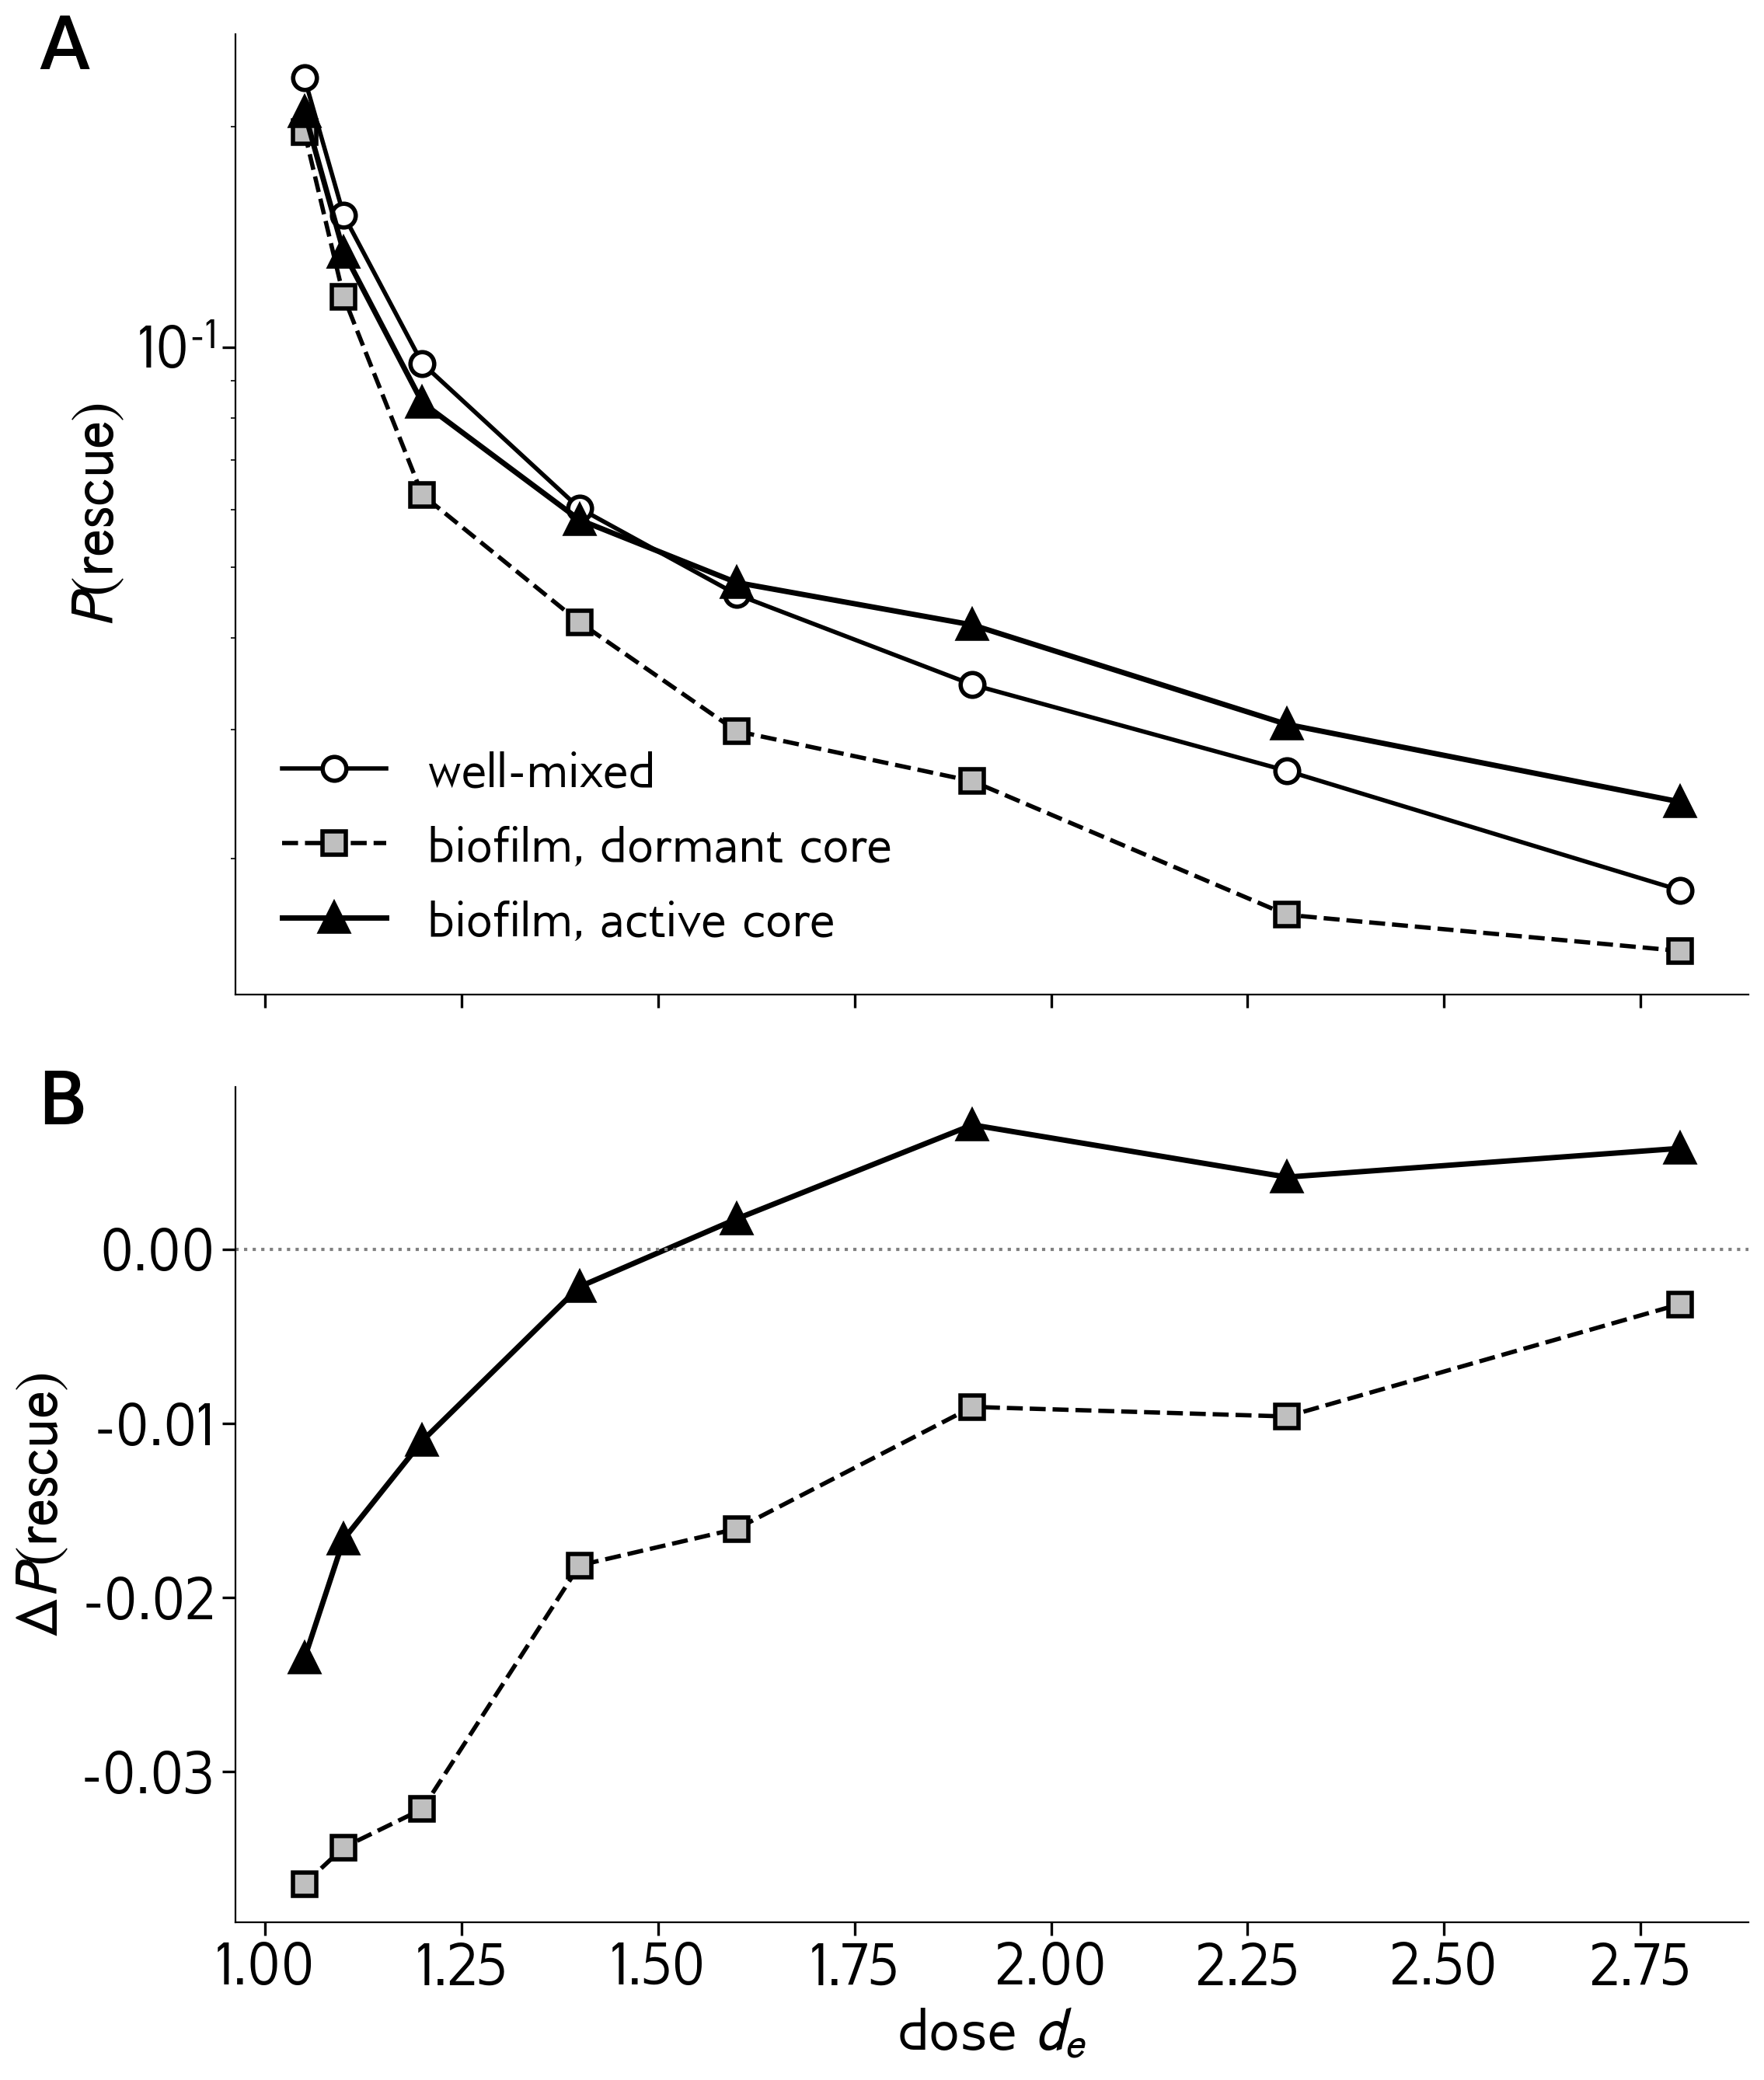
\includegraphics[width=0.75\textwidth]{dose_curves_rescue.png}
\caption{Probability of rescue versus dose for the three populations: well-mixed reference (open circles), biofilm with a dormant core ($\bCore = 0$, open squares), and biofilm with an active core ($\bCore = 0.2$, filled triangles). Panel A: absolute $P(\mathrm{rescue})$, log $y$-axis. Panel B: difference relative to the well-mixed reference, $\Delta P(\mathrm{rescue}) = P_{\mathrm{BF}} - P_{\mathrm{WM}}$, with the dotted horizontal line at zero marking the no-difference baseline. Each point averages $5{,}000$ independent simulations. \emph{Parameters}: $\Nzero = 1000$, $l = 100$, $\mu = 10^{-4}$.}
\label{fig:dosecurves}
\end{figure}

Figure~\ref{fig:decomposition} Panel A reports the first piece of the decomposition: the difference in mutation count $\Delta S = S_{\mathrm{BF}} - S_{\mathrm{WM}}$ between the biofilm and the well-mixed reference, where $S$ is the mean number of R mutations a population produces per simulation run. Two observations. First, the dormant-core biofilm sits essentially on the $y = 0$ reference line at every dose: the dormant biofilm and the well-mixed reference produce essentially the same number of mutations, even though the dormant biofilm lives longer. We return to why that extra lifetime does not translate into extra mutations in a later section. Second, the active-core biofilm sits above the $y = 0$ line at every dose: an actively dividing interior produces more mutations than the well-mixed reference at every dose. The number of extra mutations the active biofilm produces over the well-mixed reference shrinks with dose, from roughly $1.5$ extra mutations per run at $\dEdge = 1.05$ down to $\sim 0.03$ at $\dEdge = 2.8$, because the absolute number of mutations any population produces shrinks at higher dose (shorter lifetimes give fewer cell divisions during which a mutation can occur). In ratio terms, however, the active biofilm produces about $1.7\times$ as many mutations as the well-mixed reference at every dose. Notably, the number of extra mutations the active biofilm produces does not track where the biofilm wins: the largest excess in mutation count is at low dose, precisely where the active biofilm rescues less often than the well-mixed reference (Figure~\ref{fig:dosecurves} Panel B); the excess shrinks toward zero at high dose, where the biofilm actually rescues more often. Where the active biofilm has the most additional mutations available, it converts them into the fewest rescue events.

\begin{figure}[h!]
\centering
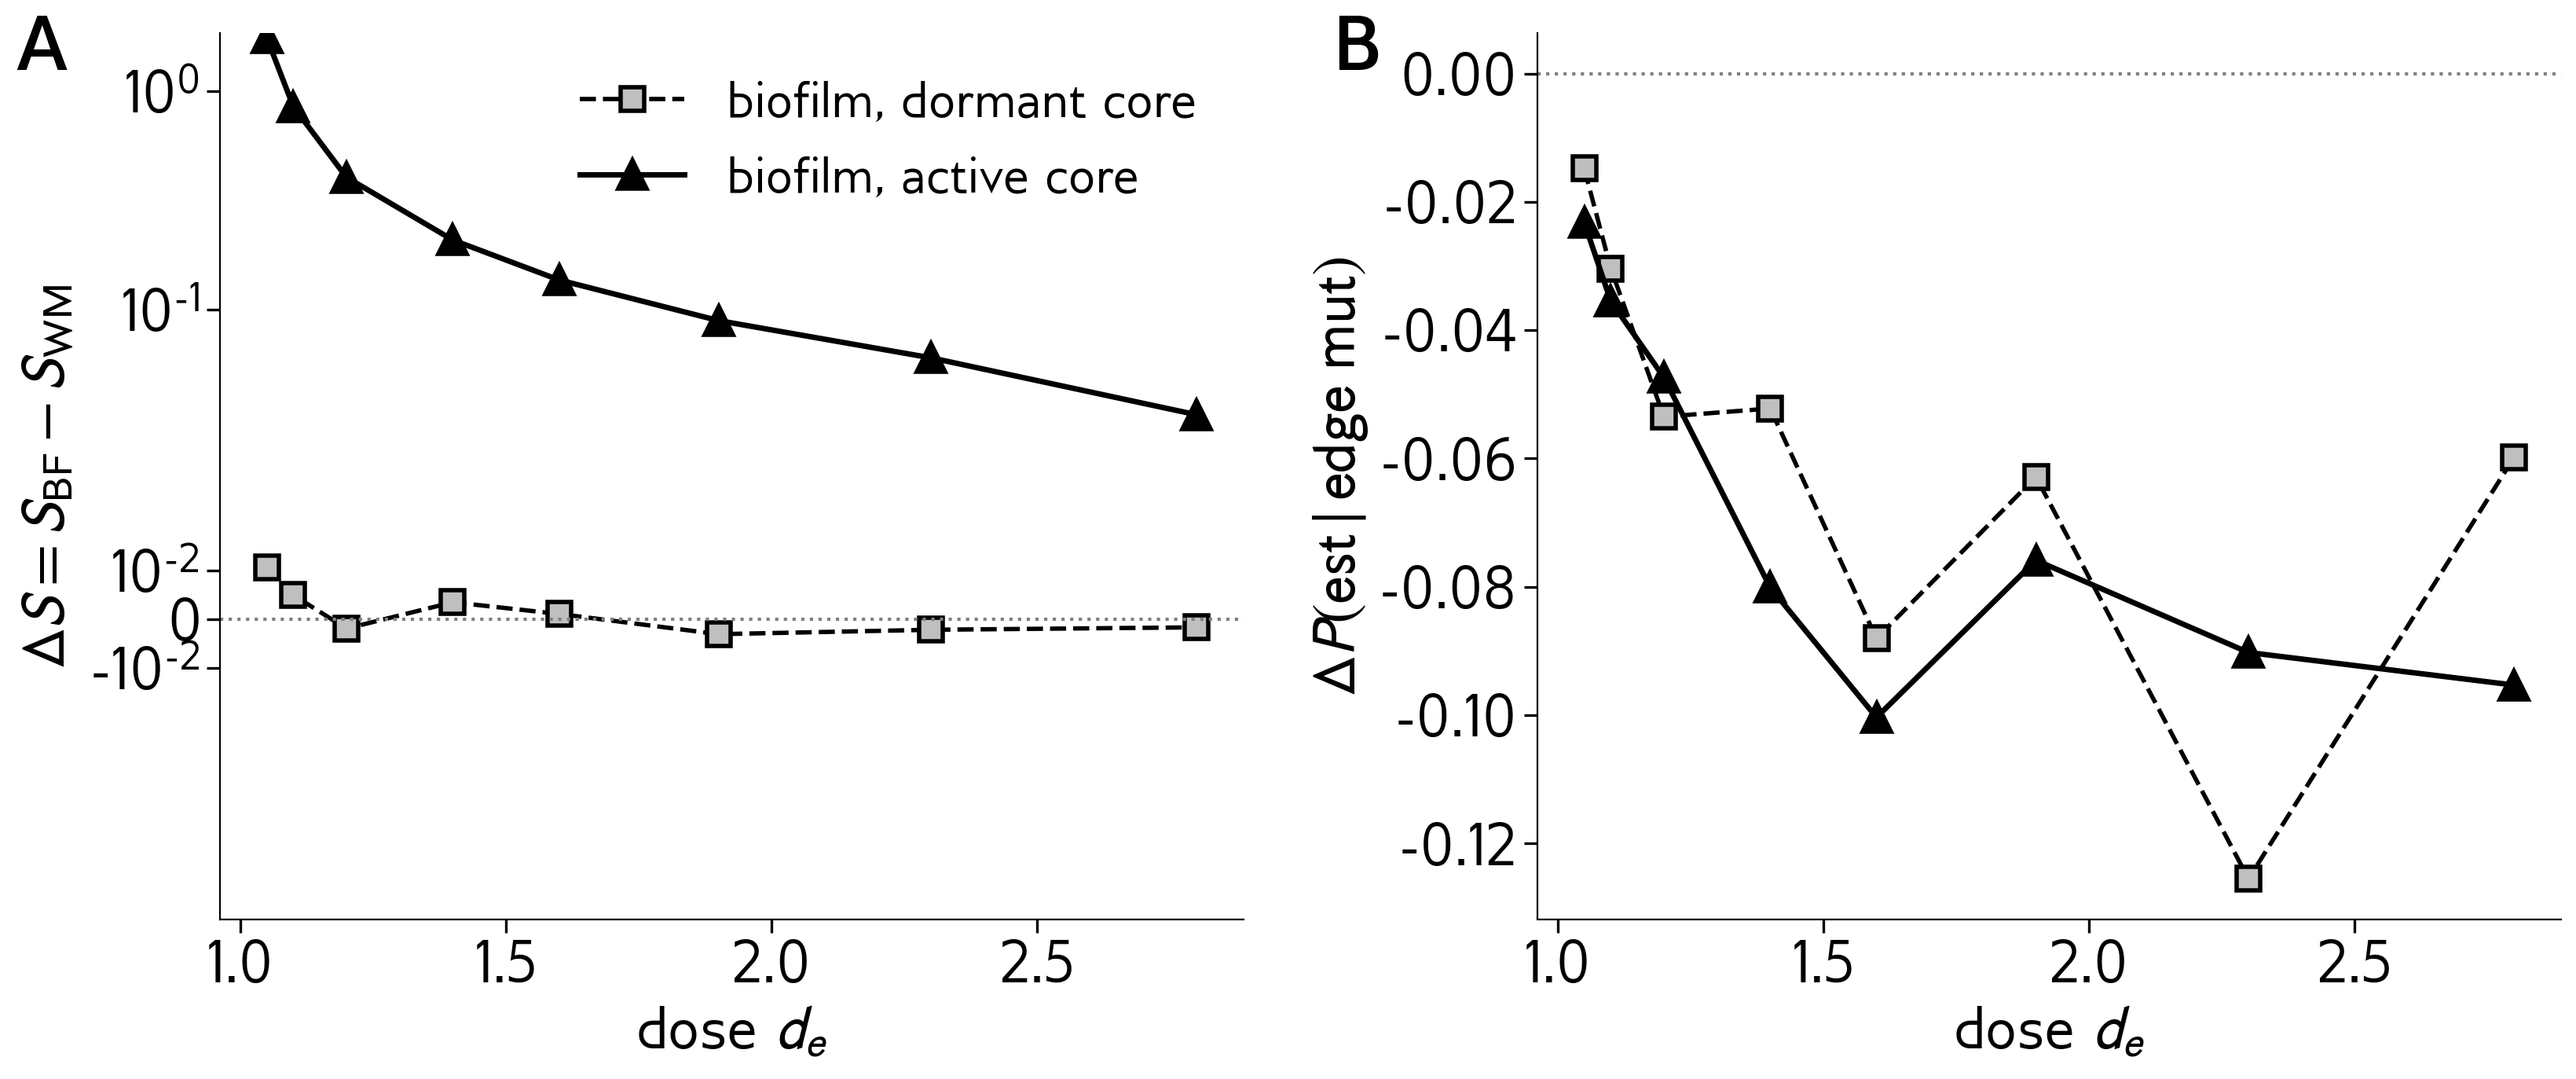
\includegraphics[width=0.95\textwidth]{decomposition.png}
\caption{Decomposing the biofilm-to-well-mixed comparison into the two ingredients rescue requires. Panel A: difference in mutation supply $\Delta S = S_{\mathrm{BF}} - S_{\mathrm{WM}}$, where $S$ is the mean number of R mutations a population produces over a simulation run. Symlog $y$-axis, with the dotted line at $y = 0$ marking equal supply. Panel B: difference in per-mutation establishment fraction for edge-born mutations, $\Delta P(\mathrm{est}) = P_{\mathrm{est},\,\mathrm{BF}} - P_{\mathrm{est},\,\mathrm{WM}}$, where $P(\mathrm{est})$ is the fraction of edge-born R lineages whose populations reach the establishment threshold $k_{\mathrm{est}} = 3$ cells before going extinct. Linear $y$-axis, with the dotted line at $y = 0$ marking equal establishment. Both panels show two biofilm conditions across the dose sweep: dormant core ($\bCore = 0$, open squares) and active core ($\bCore = 0.2$, filled triangles). Each point averages $5{,}000$ independent runs. \emph{Parameters}: $\Nzero = 1000$, $l = 100$, $\mu = 10^{-4}$.}
\label{fig:decomposition}
\end{figure}

Figure~\ref{fig:decomposition} Panel B reports the second piece: the difference in per-mutation establishment between biofilm and well-mixed, $\Delta P(\mathrm{est}) = P_{\mathrm{est},\,\mathrm{BF}} - P_{\mathrm{est},\,\mathrm{WM}}$, where $P(\mathrm{est})$ is the fraction of edge-born R lineages whose populations reach the establishment threshold $k_{\mathrm{est}} = 3$ cells before going extinct. Both biofilm curves sit below the $y = 0$ reference line at every dose: a given edge-born R lineage is consistently less likely to grow past the early-extinction bottleneck inside a biofilm than in the well-mixed reference, by roughly $0.05$ to $0.10$ in absolute probability across most of the dose range. This reduced establishment applies to both dormant and active biofilms and persists across the entire sweep. We return to why edge-born R lineages are less likely to escape early extinction inside a biofilm in a later section.

\section{Reaching the edge}
\label{sec:reachingedge}

Section~\ref{sec:supplyestab} ended on a tension. The two factors we measured (how many R mutations each population produces, and what fraction of those mutations succeed at establishing in the edge) both differ between biofilm and well-mixed in roughly dose-independent ways: the active biofilm produces about $1.8\times$ as many mutations as the well-mixed reference at every dose, and each biofilm mutation establishes about $0.8\times$ as often at every dose. Multiplied together, these two ratios predict a constant biofilm-to-well-mixed rescue ratio. The actual rescue ratio is not constant. It climbs from below $1\times$ at $\dEdge = 1.05$ to about $2\times$ at $\dEdge = 2.8$. Some dose-dependent factor that those two measurements did not capture must therefore be carrying that flip. The candidate is the one piece of the rescue calculation that the two panels of Figure~\ref{fig:decomposition} do not cover: whether a core-born R mutation ever reaches the drug-exposed edge before going extinct. The supply panel counts every R mutation a population produces, but a core-born mutation contributes to rescue only if it arrives in the edge, where antibiotic selection makes resistance an advantage. The establishment panel measures what happens to mutations once they are in the edge, but not whether they got there. Whether a given core-born R lineage actually reaches the edge is therefore a separate per-lineage outcome from either of the two pieces Section~\ref{sec:supplyestab} measured, and we measure it directly across the same dose sweep.

Figure~\ref{fig:reaching} Panel A reports this fraction directly. Two curves are shown: the default active-core biofilm ($\bCore = 0.2$, open squares) and the more active core used in Section~\ref{sec:doubleedge}'s bar plot ($\bCore = 0.8$, filled triangles). Both curves rise sharply with dose. At $\dEdge = 1.05$, only about $5$ to $10$ percent of core-born R lineages ever reach the edge; at $\dEdge = 2.8$, that fraction climbs to between $40$ and $80$ percent depending on core activity. At every dose the less active core actually has a higher fraction of core lineages reaching the edge than the more active core, an inversion we return to in the mechanism discussion below. The main point is the dose-dependent shape: in both cases the fraction rises sharply between low and high dose, matching the rescue flip in Figure~\ref{fig:dosecurves}.

\begin{figure}[h!]
\centering
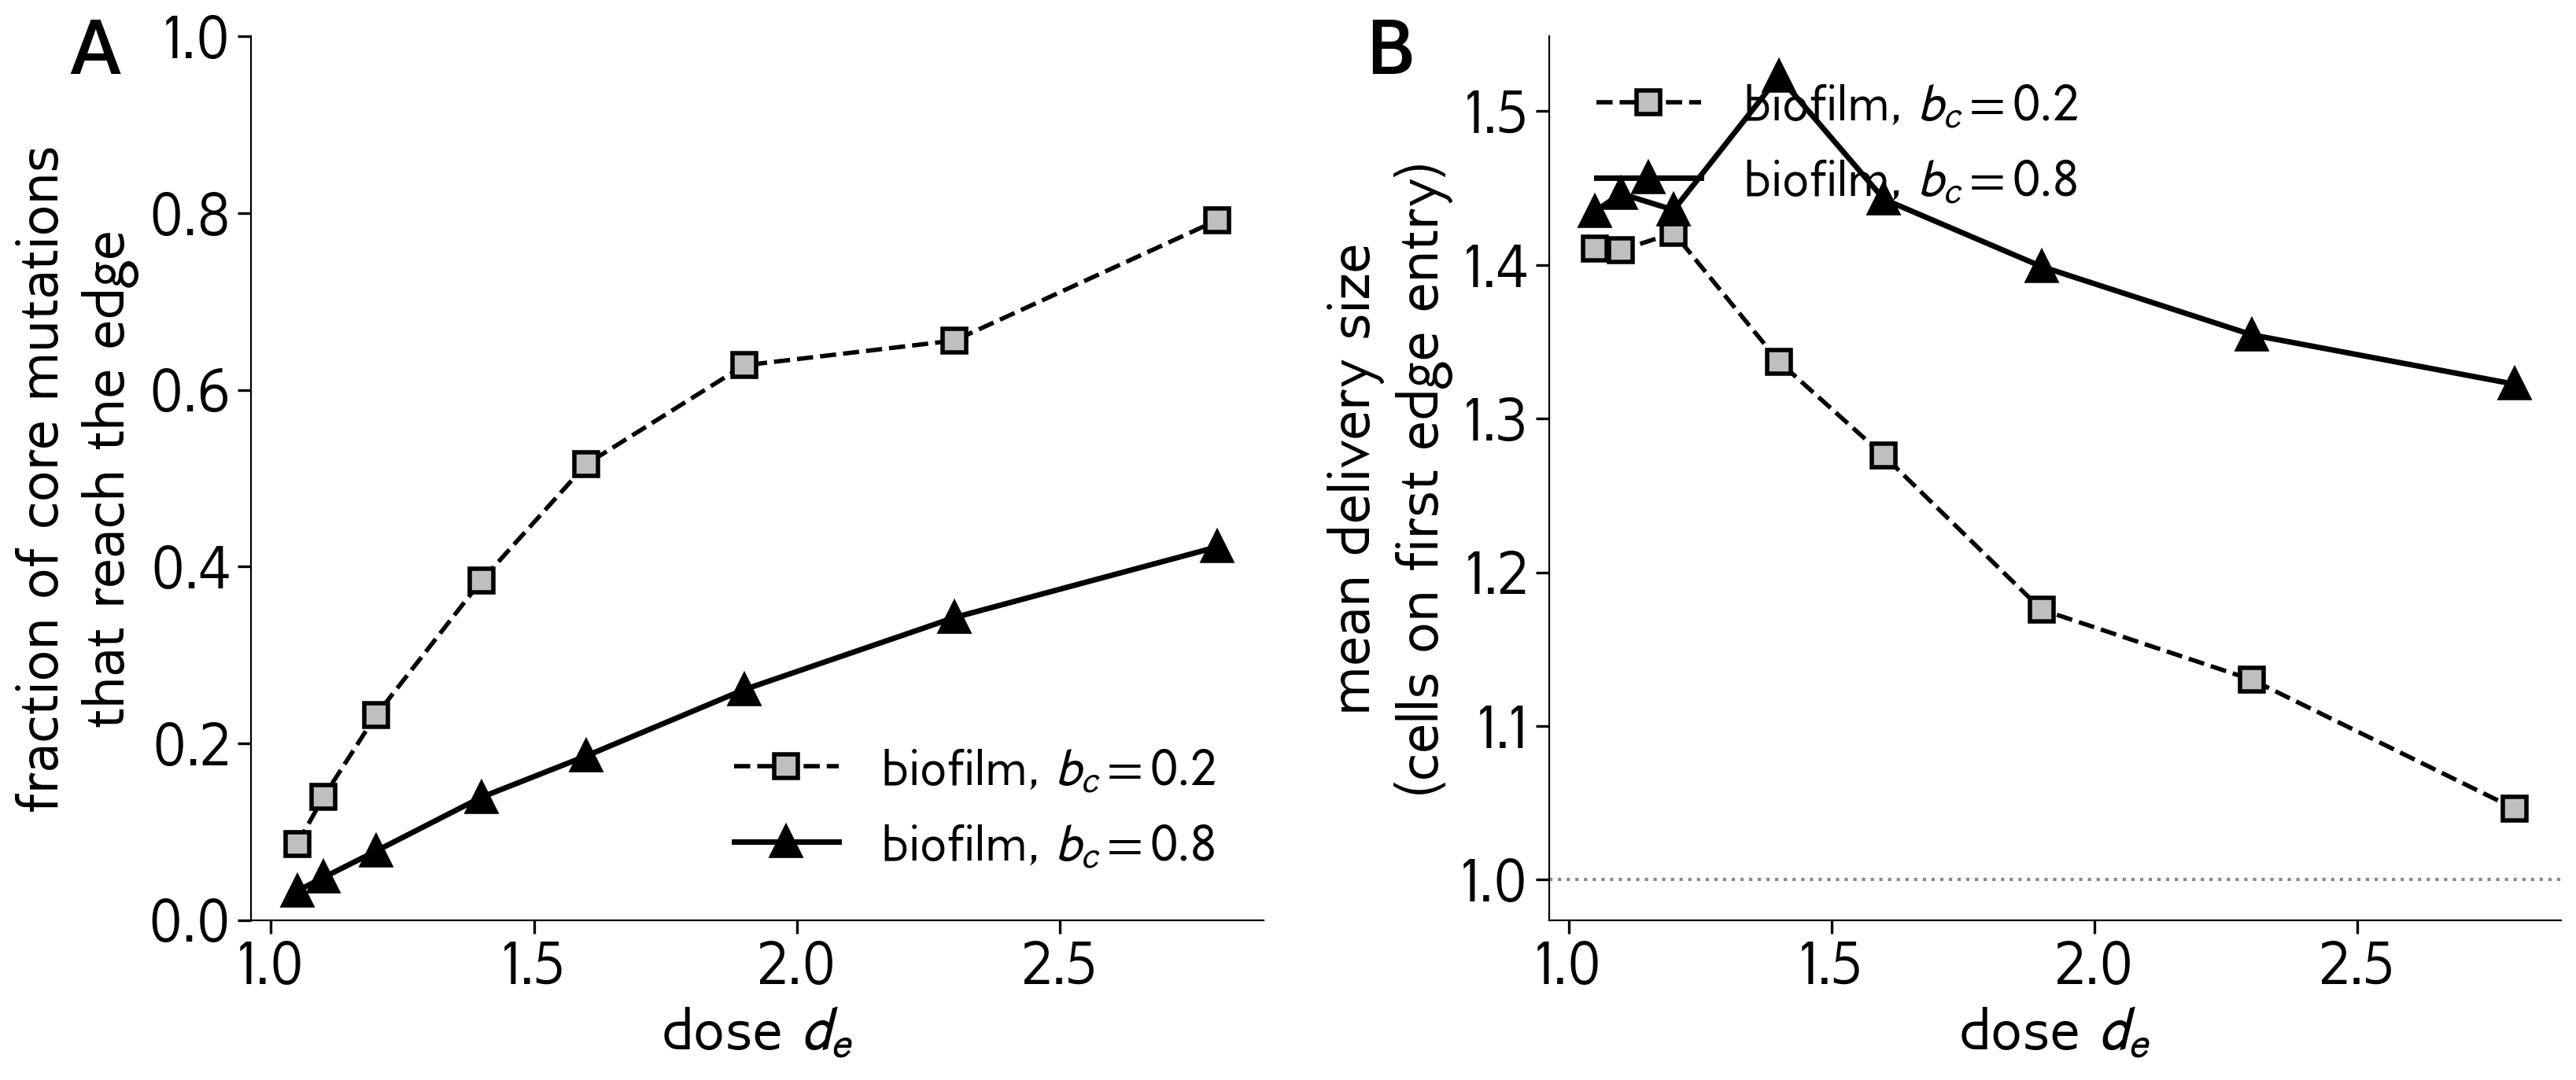
\includegraphics[width=0.95\textwidth]{delivery.png}
\caption{Per-lineage outcome of core-born R mutations. Panel A: fraction of core-born R lineages that ever reach the drug-exposed edge before going extinct, vs dose. Panel B: mean number of cells in a lineage when it first occupies an edge position, vs dose. Both panels show the default active core ($\bCore = 0.2$, open squares) and the more active core ($\bCore = 0.8$, filled triangles) used for Figure~\ref{fig:doubleedge}. Each point averages $100{,}000$ runs for $\bCore = 0.2$ and $5{,}000$ runs for $\bCore = 0.8$ per parameter combination. \emph{Parameters}: $\Nzero = 1000$, $l = 100$, $\mu = 10^{-4}$.}
\label{fig:reaching}
\end{figure}

The shape of Panel A follows from a race between two processes inside the core. A core-born R lineage starts as a single cell with balanced birth and death rates ($\bCore = \dCore$), so it does not grow on average; instead it fluctuates in size and, given enough time and turnover of cells in the core, is likely to go extinct by drift. The only way the lineage can matter for rescue is if the retreating boundary reaches its position before drift kills it. The boundary moves inward at speed $\sE \cdot l$ per unit time, where $\sE = \dEdge - \bEdge$ is the net edge death rate. At high dose, $\sE$ is large; the boundary moves inward quickly and overtakes core lineages before drift has had time to eliminate them. At low dose, $\sE$ is small; the boundary creeps inward very slowly, and most core lineages drift to extinction before they are ever exposed to the edge. The dose-dependence visible in Panel A is just this race playing out across the dose sweep, where the speed of population decline, matched with the relative size of the edge $l$, sets the time available for a core lineage to survive before the boundary catches it.

The same race explains a feature of Panel A that runs against naive expectation. At every dose, the less active core ($\bCore = 0.2$) has a higher fraction of core lineages reaching the edge than the more active core ($\bCore = 0.8$), even though the more active core produces roughly four times more core mutations per unit time. One might expect that more mutations would mean more chances for at least one to survive the race to the edge. But boundary speed and core drift are decoupled. Boundary retreat is set entirely by edge dynamics, so the time a lineage waits for the boundary to reach it is the same at $\bCore = 0.2$ as at $\bCore = 0.8$. The strength of drift in the core, however, depends directly on $\bCore$: a more active core means more births and deaths per unit time per cell, which means faster fluctuations in lineage size and faster extinction by chance. With $\bCore = 0.8$, lineages are killed in the core more quickly than at $\bCore = 0.2$, so a smaller fraction survive long enough for the boundary to reach them. The more active core produces more mutations in absolute terms, but it also kills them off faster, and the fraction surviving long enough to reach the edge drops with $\bCore$ even as the absolute mutation count rises with $\bCore$.

The dormant case is the limit of this mechanism at $\bCore = 0$. With no births in the core, no R lineages are ever born there in the first place; the race has nothing to enter. The boundary retreats at the same speed $\sE \cdot l$ as in the active case, but with no core mutations to catch, no core-born lineages ever reach the edge at any dose. The dormant biofilm therefore has no rescue advantage at any dose, not because the boundary fails to retreat, but because the core never produces a mutation for the boundary to expose to the edge in the first place.

Panel B reports a secondary consequence of the same race. The mean size of a core-born R lineage when it first arrives in the edge is slightly larger at low dose than at high dose: about $1.4$ cells per arrival at $\dEdge = 1.05$, dropping toward $1$ cell at higher dose. A lineage that survives a long wait in the core (which happens at low dose, when the boundary moves slowly) has had more time to fluctuate upward in size by chance before being caught. A lineage caught quickly (at high dose, when the boundary moves fast) is more likely to still be a single cell on first arrival. The dose dependence in Panel B runs opposite to what the rescue flip needs. A lineage arriving in the edge as a cluster of two or three cells has more independent chances to escape early extinction than a single-cell arrival: each cell can carry the lineage forward even if its siblings die. Larger clusters are therefore advantageous for establishment, and Panel B shows that larger clusters happen at low dose. If Panel B were the dominant influence on the rescue flip, the biofilm would rescue more often at low dose than at high dose. But the rescue flip goes the other way: the biofilm rescues less often at low dose and more often at high dose. Panel B therefore cannot be carrying the dose-dependence of the rescue flip.

What dominates instead is Panel A, and the reason is in the magnitudes. Panel A spans an order of magnitude across the dose range (from a few percent reaching the edge to about half reaching). Panel B varies by less than fifty percent (from about $1.4$ down to about $1.0$ cells per arrival). At low dose, the modest cluster advantage of a $1.4$-cell arrival cannot offset the fact that almost no core-born R lineages are arriving in the first place. The dose-dependence of the rescue flip therefore lives in the fraction reaching the edge at all, not in the size of those arrivals. Putting the three measurements together accounts for the rescue flip from Section~\ref{sec:doubleedge}. Rescue requires either an edge-born R mutation to establish (the path open to all populations) or a core-born R mutation to reach the edge and then establish (the path open only to biofilms with an active core). The first path is similar in biofilm and well-mixed: edge mutation counts overlap, and the per-mutation establishment fraction is only slightly reduced for the biofilm. The second path is what carries the dose-dependence.

At low dose, fewer than ten percent of core-born R lineages ever reach the edge. The active core produces more mutations overall, but those extra mutations stay trapped in the core where they cannot contribute to rescue. The biofilm therefore rescues less often than well-mixed at low dose, because the slight reduction in per-mutation establishment is no longer offset by anything from the core. At high dose, almost half of core-born R lineages reach the edge, so the active core's extra mutations now contribute a meaningful number of R lineages to the edge population, and the biofilm rescues more often than well-mixed. The crossover near $\dEdge \approx 1.4$ is where the dose-dependent reach-the-edge fraction balances the dose-independent reduction in per-mutation establishment.

The dormant case follows from the same accounting. With no core births, the second path is closed; only the first path exists, with the same edge mutation count as well-mixed and the same slightly reduced per-mutation establishment as the active biofilm. So the dormant biofilm rescues less often than well-mixed at every dose, exactly what Figure~\ref{fig:dosecurves} shows. The flip we set up in Section~\ref{sec:doubleedge} is the active biofilm's second path overtaking the first at high dose, and the dormant biofilm's lack of a second path at any dose. What remains to test is whether this account holds across the model parameters we have so far held fixed: the biofilm geometry $l$, the core activity $\bCore$, and the mutation rate $\mu$. The next section sweeps each in turn.


\section{Robustness of the rescue flip}
\label{sec:robustness}

Sections~\ref{sec:doubleedge} through~\ref{sec:reachingedge} have built and tested the rescue flip at one specific parameter combination ($\Nzero = 1000$, $l = 100$, $\mu = 10^{-4}$). A reader who has accepted the race mechanism in Section~\ref{sec:reachingedge} would reasonably ask whether the rescue flip is a robust qualitative feature of the model, or an artifact of this one setting. We sweep the three parameters held fixed in those sections (edge width $l$, core activity $\bCore$, and mutation rate $\mu$) and ask two questions of each sweep: does the flip persist across the parameter range, and does the crossover dose shift in ways the race mechanism from Section~\ref{sec:reachingedge} would predict?

Figure~\ref{fig:sensL} sweeps the edge width $l$ across $\{25, 50, 100, 200, 400\}$, holding all other parameters at their defaults. Panel A shows the dose curves for the biofilm at each $l$ alongside the well-mixed reference; Panel B shows the corresponding $\Delta P(\mathrm{rescue}) = P_{\mathrm{BF}} - P_{\mathrm{WM}}$. The flip persists across a sixteen-fold change in edge width, but its magnitude scales strongly with $l$. At smaller $l$ the flip is sharper, with the biofilm's high-dose advantage growing as $l$ shrinks: at $\dEdge = 2.8$, $\Delta P \approx 0.013$ for $l = 25$ but is essentially zero at $l = 400$, where the biofilm and well-mixed populations are indistinguishable across the entire dose range. The crossover dose itself shifts only modestly, from roughly $\dEdge \approx 1.5$ at $l = 200$ down to $\dEdge \approx 1.4$ at $l = 25$.

\begin{figure}[h!]
\centering
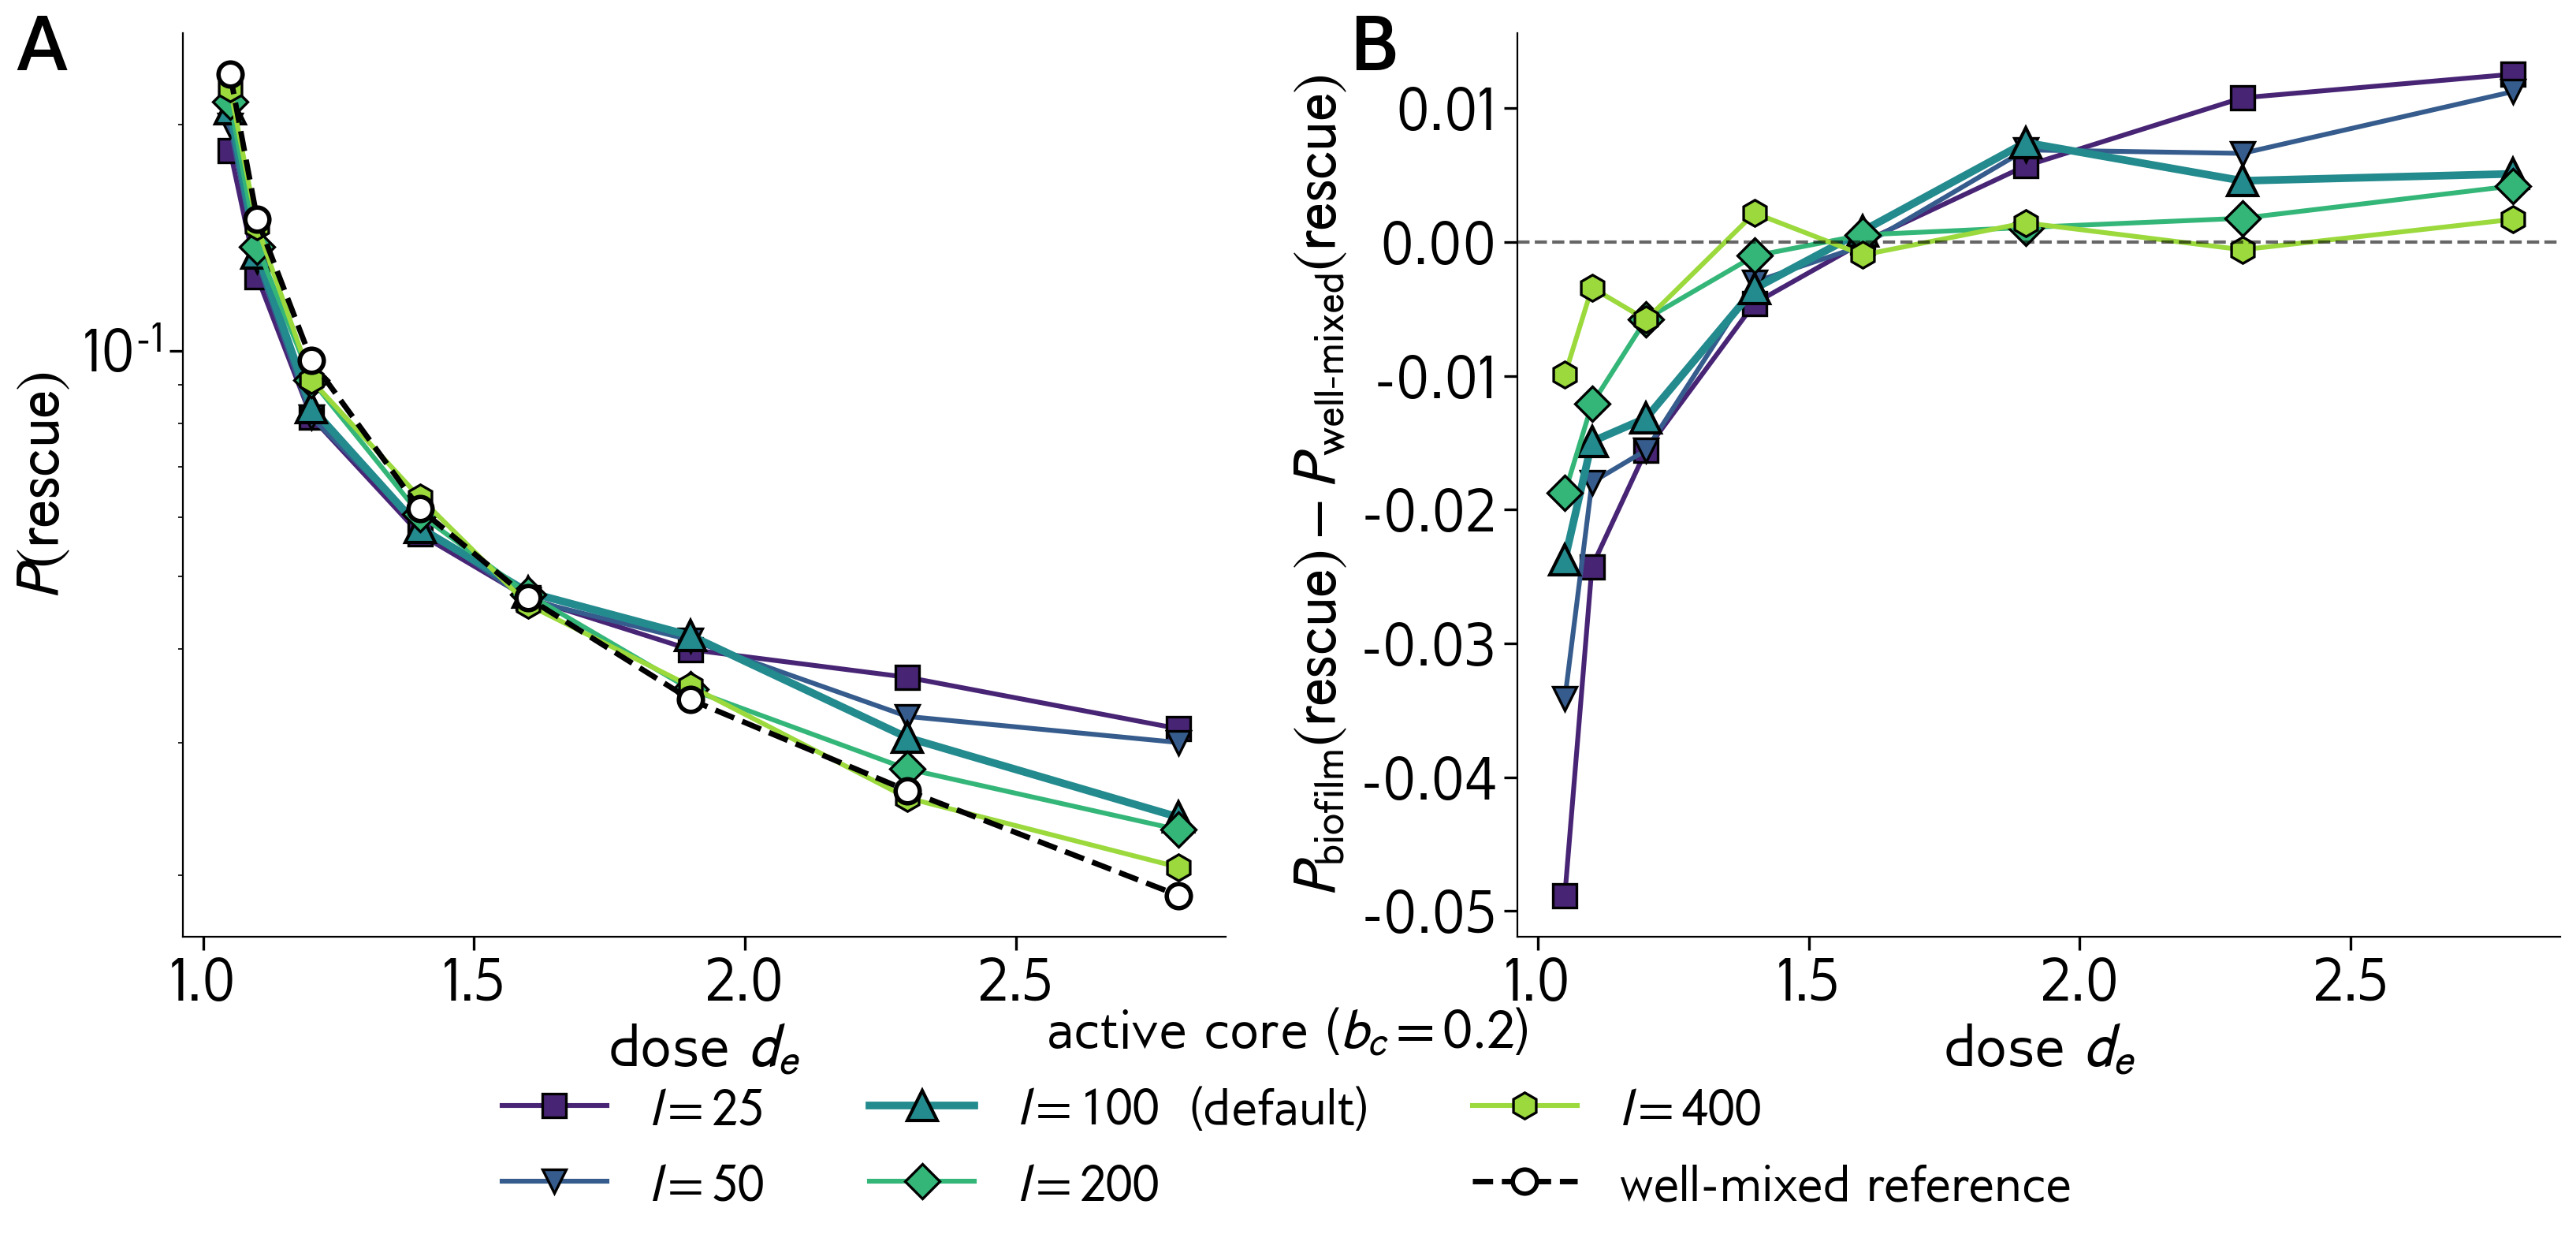
\includegraphics[width=0.95\textwidth]{sensL_curves.png}
\caption{Sensitivity of the rescue flip to edge width $l$. Panel A: $P(\mathrm{rescue})$ vs dose for the biofilm at five values of $l \in \{25, 50, 100, 200, 400\}$ and the well-mixed reference (open circles, dashed). Panel B: difference relative to the well-mixed reference, $\Delta P(\mathrm{rescue}) = P_{\mathrm{BF}} - P_{\mathrm{WM}}$, with the dotted horizontal line at zero marking the no-difference baseline. Each point averages $20{,}000$ independent simulations per parameter combination. \emph{Parameters}: $\Nzero = 1000$, $\bCore = 0.2$, $\mu = 10^{-4}$.}
\label{fig:sensL}
\end{figure}

Both shifts can be read through the race mechanism from Section~\ref{sec:reachingedge}. Smaller $l$ has two competing effects on the race. The boundary speed is $\sE \cdot l$, so smaller $l$ slows boundary retreat in absolute cell terms, which by itself would reduce the fraction of core mutations that reach the edge. But smaller $l$ also makes the core larger relative to the total population (it is $\Nzero - l$ cells), which means more core births per unit time and a longer Phase 1 over which to produce them: the duration $T_1 = (\Nzero - l) / (\sE \cdot l)$ increases as $l$ decreases. The larger pool of core mutations more than compensates for the slower boundary retreat. The net effect tilts the race toward the biofilm at smaller $l$, which is what Panel B shows.

Figure~\ref{fig:sensCore} sweeps the core metabolic activity $\bCore$ across $\{0, 0.05, 0.1, 0.2, 0.4, 0.8\}$, holding all other parameters at their defaults. Panel A shows the dose curves for the biofilm at each $\bCore$ alongside the well-mixed reference; Panel B shows the corresponding $\Delta P(\mathrm{rescue})$. At $\bCore = 0$ (dormant core), the biofilm stays strictly below the well-mixed reference at every dose; there is no crossover. At every $\bCore > 0$ in the sweep, the biofilm crosses the well-mixed reference at some dose and stays at or above it at higher doses. The crossover dose shifts predictably with $\bCore$: from $\dEdge \approx 1.6$ at $\bCore = 0.05$ down to $\dEdge \approx 1.2$ at $\bCore = 0.8$. The high-dose advantage also grows with $\bCore$: at $\dEdge = 2.8$, $\Delta P$ at $\bCore = 0.8$ is about four times its value at $\bCore = 0.05$.

\begin{figure}[h!]
\centering
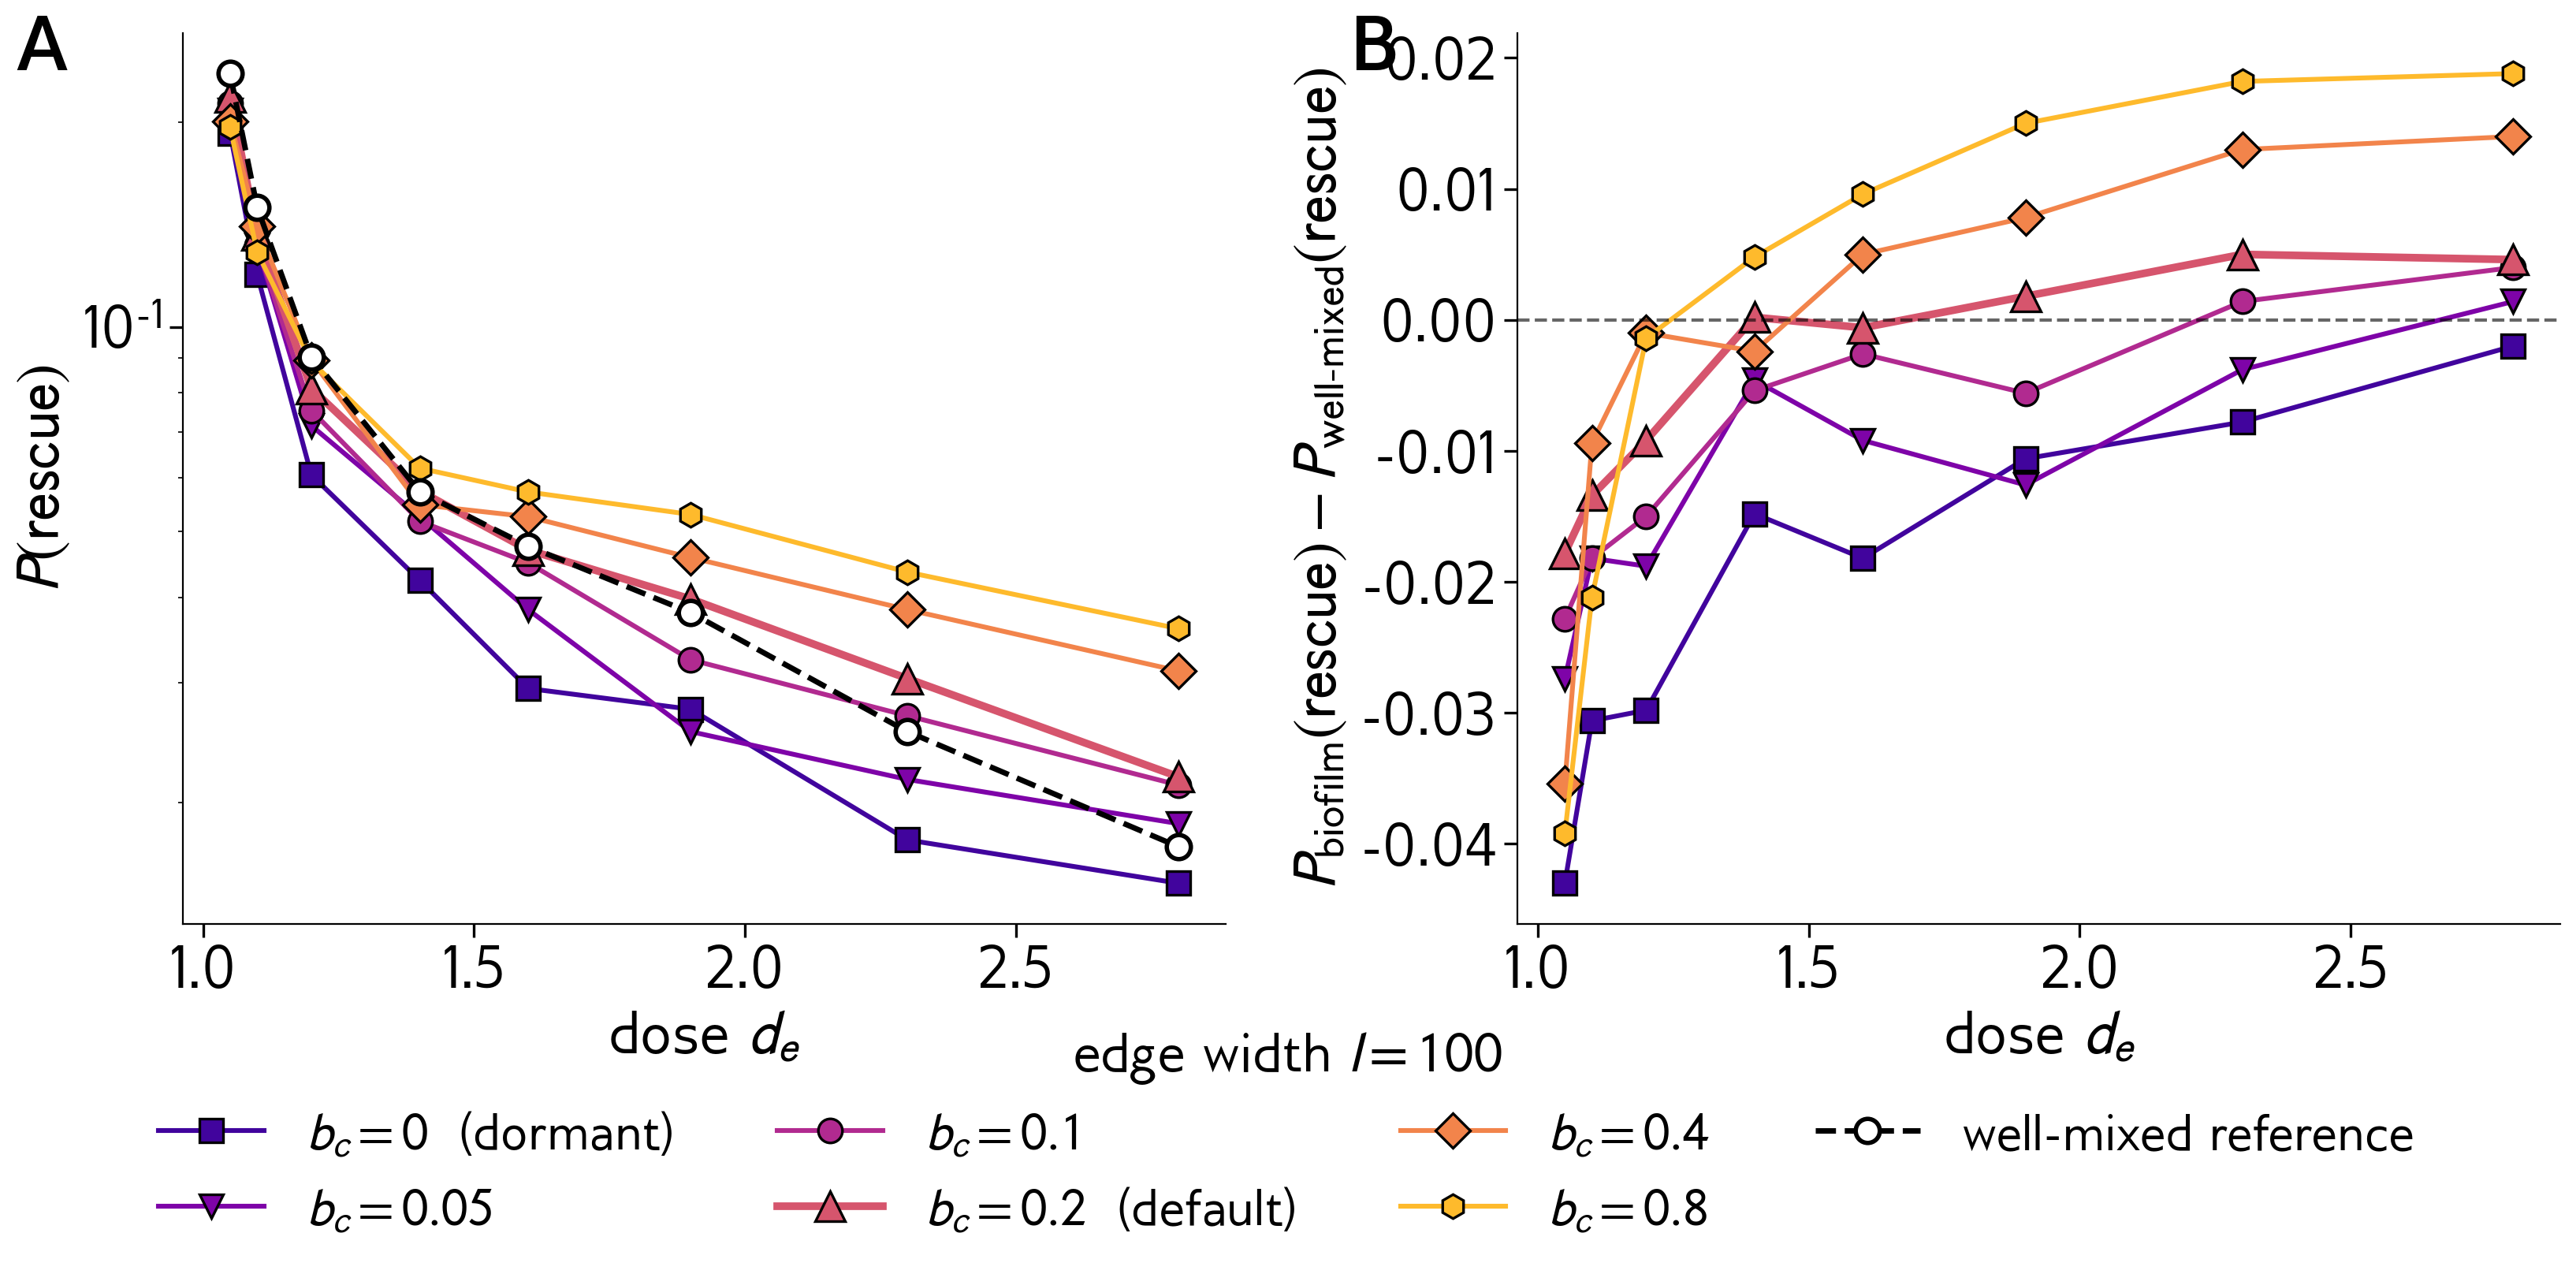
\includegraphics[width=0.95\textwidth]{sensCore_curves.png}
\caption{Sensitivity of the rescue flip to core metabolic activity $\bCore$. Panel A: $P(\mathrm{rescue})$ vs dose for the biofilm at six values of $\bCore \in \{0, 0.05, 0.1, 0.2, 0.4, 0.8\}$ and the well-mixed reference (open circles, dashed). Panel B: difference relative to the well-mixed reference, $\Delta P(\mathrm{rescue}) = P_{\mathrm{BF}} - P_{\mathrm{WM}}$, with the dotted horizontal line at zero marking the no-difference baseline. Each point averages $20{,}000$ independent simulations per parameter combination. \emph{Parameters}: $\Nzero = 1000$, $l = 100$, $\mu = 10^{-4}$.}
\label{fig:sensCore}
\end{figure}

The shifts can be read through the race mechanism from Section~\ref{sec:reachingedge}. The dormant case ($\bCore = 0$) is the cleanest test: with no core births, no R lineages are ever produced in the core for the boundary to catch, and the biofilm gains no advantage at any dose. The $\bCore > 0$ cases trade off two effects of increasing the core's metabolic rate. Higher $\bCore$ produces more core mutations per unit time, which feeds more lineages into the race. But higher $\bCore$ also accelerates drift in the core, so a smaller fraction of those lineages survive long enough for the boundary to reach them (Figure~\ref{fig:reaching} showed this directly: at $\bCore = 0.8$, fewer core lineages reach the edge as a fraction than at $\bCore = 0.2$). The absolute mutation count rises faster than the fraction lost, so the total flow of core lineages arriving at the edge increases with $\bCore$, and the biofilm's high-dose advantage grows accordingly.

Figure~\ref{fig:sensMu} sweeps the mutation rate $\mu$ across $\{10^{-5}, 10^{-4}, 10^{-3}\}$, holding all other parameters at their defaults. Mutation rate scales the absolute rescue probability strongly: at $\mu = 10^{-3}$ both populations rescue close to a substantial fraction of the time at low dose, while at $\mu = 10^{-5}$ rescue is rare for both at every dose. The qualitative flip persists at $\mu = 10^{-4}$ (our default, with crossover at $\dEdge \approx 1.4$) and at $\mu = 10^{-3}$ (crossover at $\dEdge \approx 1.5$, with the high-dose advantage about an order of magnitude larger than at the default $\mu$). At $\mu = 10^{-5}$, both populations rescue so rarely that the absolute $\Delta P$ stays near zero across the sweep; resolving the flip cleanly at this mutation rate would require many more replicates than we have. Within the range where the model produces measurable rescue events, the qualitative shape of the flip is robust to $\mu$: the mutation rate sets how often any rescue happens, but does not change which population gets the larger flow of core-born lineages arriving at the edge at high dose.

\begin{figure}[h!]
\centering
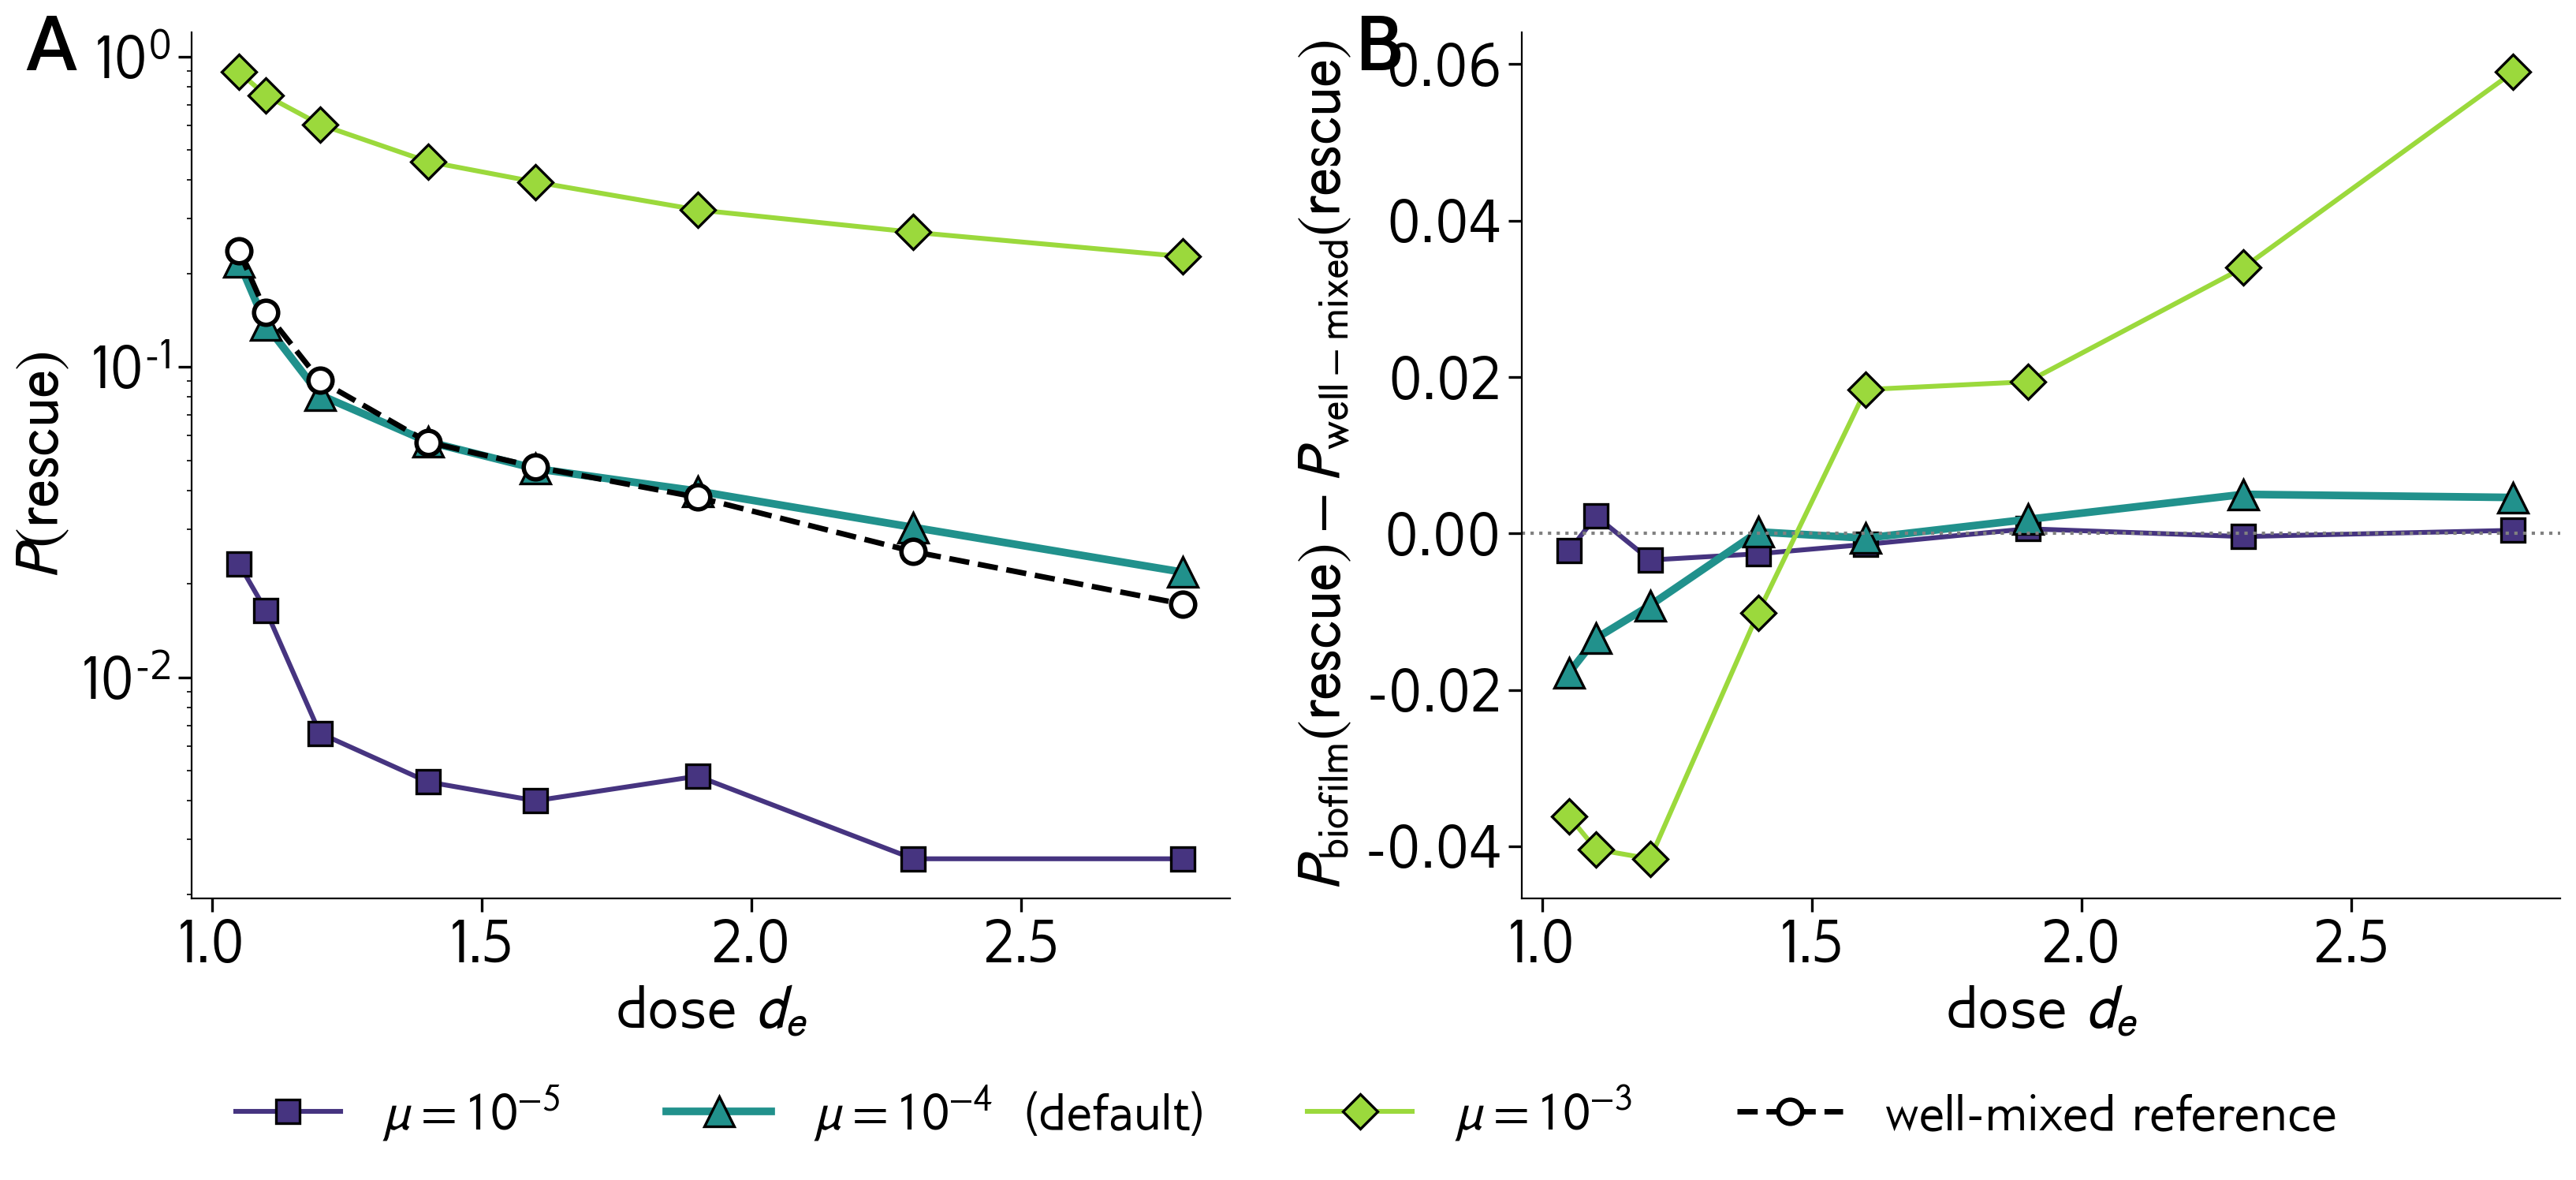
\includegraphics[width=0.95\textwidth]{sensMu_curves.png}
\caption{Sensitivity of the rescue flip to mutation rate $\mu$. Panel A: $P(\mathrm{rescue})$ vs dose for the biofilm at three values of $\mu \in \{10^{-5}, 10^{-4}, 10^{-3}\}$ and the well-mixed reference at $\mu = 10^{-4}$ (open circles, dashed). Panel B: difference relative to the well-mixed reference at each $\mu$, $\Delta P(\mathrm{rescue}) = P_{\mathrm{BF}} - P_{\mathrm{WM}}$, with the dotted horizontal line at zero. Each point averages $20{,}000$ independent simulations per parameter combination. \emph{Parameters}: $\Nzero = 1000$, $l = 100$, $\bCore = 0.2$.}
\label{fig:sensMu}
\end{figure}

Across all three sweeps, the rescue flip is a robust qualitative feature of the model. The flip persists at every edge width $l$ we tested (a sixteen-fold change in $l$), at every nonzero core activity $\bCore$, and at every mutation rate $\mu$ for which the model produces measurable rescue events. The locations of the flip (the crossover doses) shift in directions that the race mechanism from Section~\ref{sec:reachingedge} predicts: changes in $l$ alter both the boundary speed and the duration of Phase 1, changes in $\bCore$ alter both how many core mutations are produced and how fast they drift to extinction, and changes in $\mu$ scale the overall mutation supply without changing the race dynamics. The biofilm wins where these factors combine to produce a flow of core lineages arriving at the edge large enough to overcome the biofilm's per-mutation establishment penalty.

Sections~\ref{sec:doubleedge} through~\ref{sec:robustness} have now built the rescue flip, measured its mechanism, and tested its robustness across the three parameters that govern it. What remains is the question Section~\ref{sec:intro} actually opened with: what does this tell us about treating biofilm infections, and in particular about behavior-modifying interventions that disrupt biofilm spatial structure? The next section returns to that motivating question with the mechanism in hand.


% Sections to come (placeholders, not yet drafted):
%   07: clinical / biological implications (closing the loop on §1)
%   06: supply mechanism (lifetime vs cell-time; active-core bonus)
%   07: delivery (drift-limited core delivery; bolus)
%   08: per-mutation tax (conveyor belt + density factor)

\end{document}
